%==============================================================================
% Reduced-Sector chi-Universality in Lorentzian EC+NY Minisuperspace:
% Topology-Robust Admissibility, P-Channel Diagnostics,
% and Reduced Vacuum Orbits
%==============================================================================
\documentclass[12pt,a4paper]{article}

%------------------------------------------------------------------------------
% Packages
%------------------------------------------------------------------------------

% Fonts / encoding
\usepackage[T1]{fontenc}
\usepackage{lmodern}
\usepackage{textcomp}
\usepackage[final]{microtype}

% Math
\usepackage{amsmath,amssymb,amsfonts,amsthm}
\usepackage{mathtools}
\usepackage{bm}

% Graphics and figures
\usepackage{graphicx}
\usepackage{float}
\usepackage{subcaption}

% Tables
\usepackage{booktabs}
\usepackage{tabularx}
\usepackage{array}
\usepackage{multirow}
\usepackage{longtable}
\usepackage{xurl}

\newcolumntype{Y}{>{\raggedright\arraybackslash}X}
\newcommand{\code}[1]{\path{#1}}
\newcolumntype{L}[1]{>{\raggedright\arraybackslash}p{#1}}

% Layout and formatting
\usepackage[margin=2.5cm]{geometry}
\usepackage{setspace}
\onehalfspacing

% Misc (xcolor before hyperref)
\usepackage{xcolor}
\usepackage{enumitem}

% References and links
\definecolor{linkblue}{RGB}{0,0,180}
\usepackage[colorlinks=true,linkcolor=linkblue,citecolor=linkblue,urlcolor=linkblue]{hyperref}
\usepackage{cleveref}

% Code listings
\usepackage{listings}
\lstset{
  basicstyle=\ttfamily\small,
  breaklines=true,
  frame=single,
  language=Python
}

% Section break
\usepackage{titlesec}
\newcommand{\sectionbreak}{\clearpage}

%------------------------------------------------------------------------------
% Theorem environments
%------------------------------------------------------------------------------
\newtheorem{theorem}{Theorem}
\newtheorem{proposition}{Proposition}
\newtheorem{lemma}{Lemma}
\newtheorem{corollary}{Corollary}
\theoremstyle{definition}
\newtheorem{definition}{Definition}
\theoremstyle{remark}
\newtheorem{remark}{Remark}

%------------------------------------------------------------------------------
% Custom commands
%------------------------------------------------------------------------------
% Math shortcuts
\newcommand{\dd}{\mathrm{d}}
\newcommand{\Sthree}{S^{3}}
\newcommand{\Tthree}{T^{3}}
\newcommand{\Nilthree}{\mathrm{Nil}^{3}}
\newcommand{\Solthree}{\mathrm{Sol}^{3}}
\newcommand{\kap}{\kappa}

% Topology bookkeeping
\newcommand{\topo}{\Sigma}
\newcommand{\Ctop}{C_{\mathrm{topology}}}
\newcommand{\Disc}{\Delta}

% Diagnostic quantities
\newcommand{\Pform}{P_{\mathrm{form}}}
\newcommand{\Pint}{P_{\mathrm{int}}}
\newcommand{\PintMX}{P_{\mathrm{int}}^{\mathrm{MX}}}
\newcommand{\QNY}{Q_{\mathrm{NY}}}
\newcommand{\thetaNY}{\theta_{\mathrm{NY}}}

% Branch labels
\newcommand{\EH}{\mathrm{EH}}
\newcommand{\AX}{\mathrm{AX}}
\newcommand{\VT}{\mathrm{VT}}
\newcommand{\MX}{\mathrm{MX}}

% Hamiltonian
\newcommand{\Ham}{\mathcal{H}}

% Geometry
\newcommand{\Vol}{\mathcal{V}}
\newcommand{\tr}{\mathrm{tr}}
\newcommand{\Tr}{\mathrm{Tr}}

%------------------------------------------------------------------------------
% Title and author
%------------------------------------------------------------------------------
\title{Reduced-Sector $\chi$-Universality\\in Lorentzian EC+NY Minisuperspace:\\
Topology-Robust Admissibility, P-Channel Diagnostics,\\
and Reduced Vacuum Orbits}

\author{Muacca}

\date{}

%==============================================================================
\begin{document}
%==============================================================================

\maketitle
\begin{center}
Version: v1\\
First release: 2026-05-16
\end{center}

%------------------------------------------------------------------------------
% Abstract
%------------------------------------------------------------------------------
\begin{abstract}
We analyse the topology dependence of the Lorentzian Einstein--Cartan plus
Nieh--Yan (EC+NY) reduced sector across the four homogeneous three-geometries
$\Sthree$, $\Tthree$, $\Nilthree$, and $\Solthree$, restricted to the
$\alpha=0$ EC+NY reduced branch.  For $\Nilthree$ and $\Solthree$ the
treatment is confined to the isotropic-scale reduction.

In this reduced sector the Hamiltonian constraint and the torsion auxiliary
equations exhibit a topology-robust admissibility pattern: the EH, AX, and VT
branches are admissible, while the MX branch is conditionally admissible
through a real auxiliary branch.  For Pontryagin-type quantities we separate
the form-Hodge density $\Pform$, the internal-pair diagnostic $\Pint$, and the
Nieh--Yan endpoint channel $\QNY$.  The form-Hodge density $\Pform$ vanishes
exactly on the active torsion branches by block orthogonality.  The
diagnostic $\Pint$ on the MX branch carries the topology dependence in a
single coefficient, $\Ctop = -9\chi$.

Furthermore, the reduced vacuum orbit atlas on the auxiliary shell reduces to
$\dot q^{2} + \chi = 0$.

Consequently, $\chi>0$ admits no real initial data on the reduced vacuum
atlas, $\chi=0$ gives static or degenerate behaviour, and $\chi<0$ gives
monotonic expansion together with singular-approach collapse sheets.

The two relations $\Ctop=-9\chi$ and $\dot q^{2}+\chi=0$ are obtained from
independent computational routes and converge on the same scalar $\chi$;
this convergence is the content of the $\chi$-controlled topology
universality.  The results are a classification within the reduced
Lorentzian EC+NY sector; global, anisotropic, and matter-coupled extensions
are left to future work.
\end{abstract}

%------------------------------------------------------------------------------
% Main text
%------------------------------------------------------------------------------
%==============================================================================
% Section 1: Introduction
%==============================================================================
\section{Introduction}
\label{sec:intro}

\subsection{Background and motivation}
\label{sec:intro:background}

The DPPU series has progressively organised the Einstein--Cartan plus
Nieh--Yan setting~\cite{Hehl1976,NiehYan1982} in terms of homogeneous
geometries, torsion modes, Pontryagin-type diagnostics, and topology
response~\cite{paper1,paper2,paper3,paper3ec,paper4}.  Paper~V~\cite{paper5}
constructed the $\alpha=0$ EC+NY baseline in Lorentzian signature on the
$\Sthree$ closed-FLRW branch, and established the channel separation among the
Hamiltonian constraint, the torsion auxiliary sector, and the diagnostic
quantities $\Pform$, $\Pint$, and $\QNY$.

The aim of the present paper is to extend that baseline to the four
topologies
\begin{equation}
  \Sthree, \quad \Tthree, \quad \Nilthree, \quad \Solthree,
\end{equation}
and to make explicit how topology dependence appears in the branch
classification and in the diagnostic structure.  The subject of this paper
is not bounce cosmology model building, but a classificatory analysis of
$\chi$-controlled topology universality in the reduced sector.

\subsection{Main results}
\label{sec:intro:results}

The main results of this paper are the following.

\begin{enumerate}
  \item In the Lorentzian EC+NY reduced setting, the four topologies
        $\Sthree$, $\Tthree$, $\Nilthree$, and $\Solthree$ share the same
        local admissibility pattern: $\EH$, $\AX$, and $\VT$ are admissible,
        while $\MX$ is conditionally admissible.

  \item On the active torsion branches, $\Pform$ vanishes exactly by block
        orthogonality.

  \item $\PintMX$ has a topology-universal functional template; the
        topology dependence is localised in the single coefficient
        $\Ctop = -9\chi$.

  \item $\QNY$ is an endpoint or boundary channel: zero on $\VT$,
        on-shell trivial on $\AX$, and boundary-conditional on $\MX$.

  \item On the auxiliary shell, the reduced vacuum orbit is governed by
        $\dot q^{2}+\chi=0$.

  \item Within this vacuum reduced atlas, no bounce-like or
        recollapse-like orbit class is found.
\end{enumerate}

The scalar $\chi$ in result~3 and in result~5 is obtained from independent
routes -- a symbolic analysis of $\PintMX$ and a derivation from the
$\EH$-spatial-curvature sector, respectively -- and the agreement of these
two routes is the substance of $\chi$-universality.

In other words, in the Lorentzian EC+NY reduced sector topology does not
alter the algebraic admissibility pattern, but controls the MX internal
diagnostic and the vacuum auxiliary-shell orbit through the same scalar
$\chi$.

\begin{figure}[H]
  \centering
  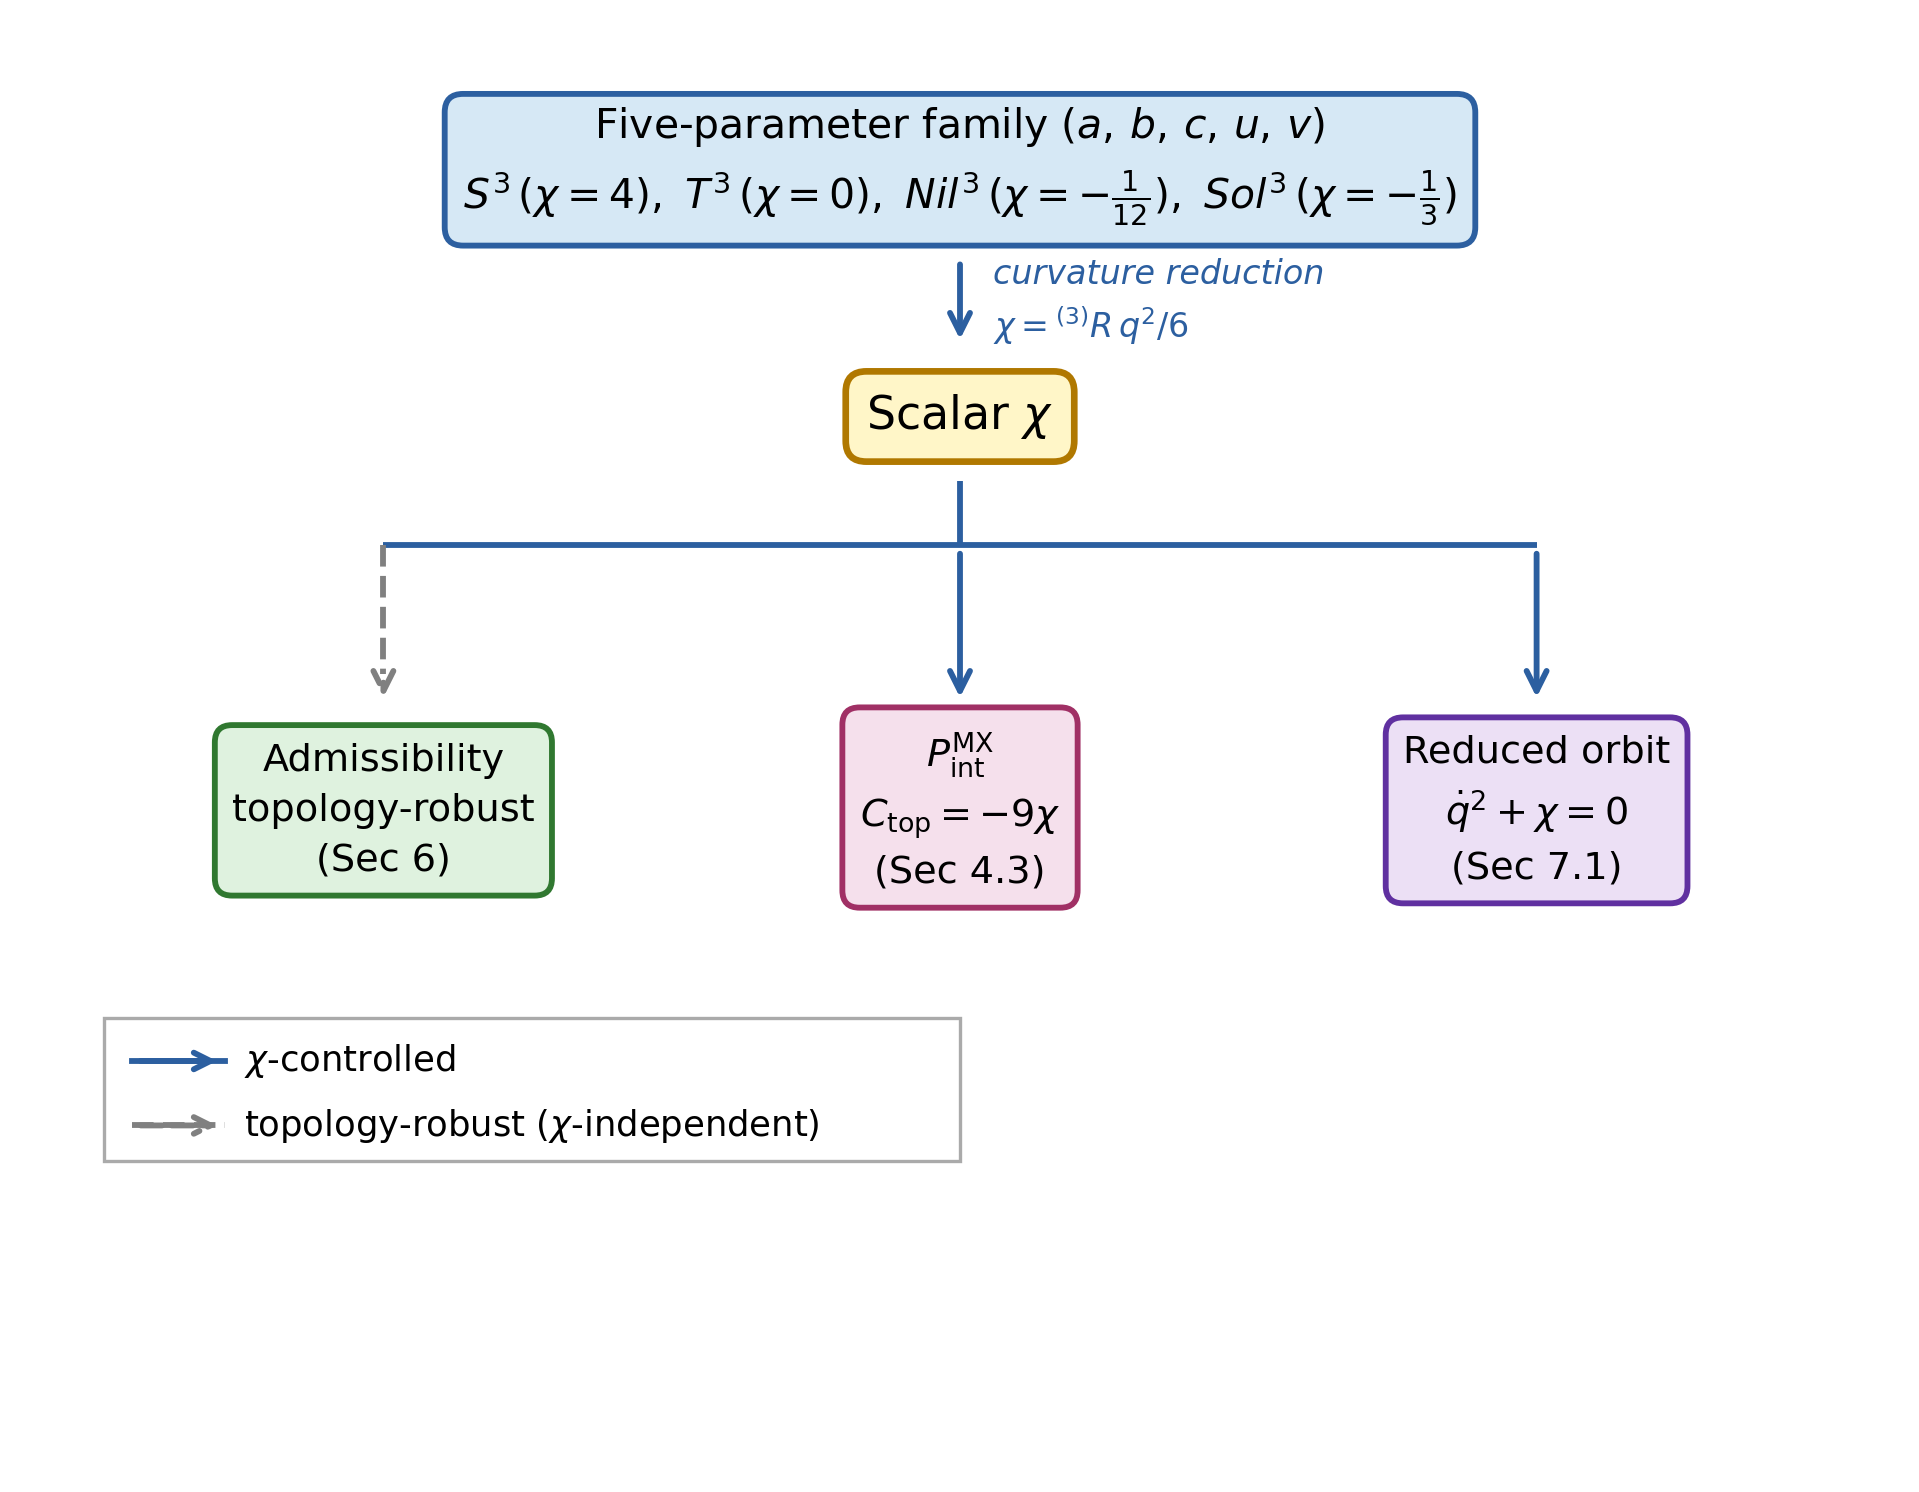
\includegraphics[width=0.9\textwidth]{figures/fig01_three_level_architecture.png}
  \caption{Three-level architecture of $\chi$-controlled topology
    universality in the reduced LZ-native isotropic EC+NY sector.  The
    five-parameter family $(a,b,c,u,v)$ at the top reduces, via the
    spatial-curvature contraction, to the scalar $\chi$, from which three
    independent consequences follow: the topology-robust admissibility
    pattern, the MX diagnostic identity $\Ctop=-9\chi$, and the reduced
    vacuum orbit $\dot q^{2}+\chi=0$.  The arrow to admissibility (dashed)
    indicates that the admissibility pattern does not depend on $\chi$.
    The arrows to $\PintMX$ and to the reduced orbit (solid) indicate
    $\chi$-mediated control.  \emph{Scope}: limited to the reduced
    LZ-native isotropic EC+NY sector; global, anisotropic, and
    matter-coupled extensions lie outside the scope of this paper.}
  \label{fig:three_level_architecture}
\end{figure}

\subsection{Relation to earlier DPPU papers}
\label{sec:intro:relation}

Paper~V~\cite{paper5} constructed the Lorentzian $\alpha=0$ EC+NY baseline on
$\Sthree$ and separated $\Pform$ from $\Pint$.  The present paper extends
that baseline to a four-topology table.

In particular, the $\Sthree$ row of the present paper reproduces the
$\alpha=0$ Lorentzian baseline of paper~V.  In Table~B1, the $\Sthree$ entry
has $F_{\mathrm{shell}}=4$, the $\MX$ auxiliary Hessian
$-4q^{2}(\kap^{4}\thetaNY^{2}+1)/9$, and the classification label
\code{L_CONDITIONALLY_ADMISSIBLE}.  The new content of the present paper is
that the same pattern extends to $\Tthree$, $\Nilthree$, and $\Solthree$.

In paper~IV~\cite{paper4} the same four Thurston
geometries~\cite{Thurston1997,Scott1983} produced four response types -- none,
uniaxial, triaxial, and biaxial -- in the Euclidean response dictionary.  As
discussed in Section~\ref{sec:bridge:loci}, the same four geometries reappear
here as structurally distinguished loci in the LZ-native isotropic
five-parameter family.  This correspondence is a structural resonance, and
its interpretation is taken up in Section~\ref{sec:discussion:paper04echo}.

\subsection{Organisation of the paper}
\label{sec:intro:outline}

Section~\ref{sec:setup} fixes the Lorentzian-native setup and the topology
conventions.
Section~\ref{sec:hamiltonian} states the Hamiltonian admissibility backbone.
Section~\ref{sec:pchannel} organises the channel dictionary for $\Pform$,
$\Pint$, and $\QNY$.
Section~\ref{sec:bridge} connects the diagnostic-level and reduced-orbit-level
$\chi$-universality.
Section~\ref{sec:classification} summarises the four-topology admissibility
classification.
Section~\ref{sec:orbit} states the reduced orbit atlas and the
$\chi$-sign separation.
Section~\ref{sec:discussion} discusses the meaning of $\chi$-universality,
the relation to paper~IV, and future directions.
Appendix~\ref{app:A} supplements the topology conventions, local reductions,
and caveats.
Appendix~\ref{app:B} collects tables, computational checks, and
reproducibility notes.
Appendix~\ref{app:C} states a Bianchi~I lite comparison and the reduced-atlas
scope guard.
   % Introduction
%==============================================================================
% Section 2: Lorentzian-native setup and topology conventions
%==============================================================================
\section{Lorentzian-native setup and topology conventions}
\label{sec:setup}

\subsection{Reduced Lorentzian frame}
\label{sec:setup:frame}

We use the orthonormal frame of Lorentzian signature $(-,+,+,+)$.  The
coframe is written as
\begin{equation}
  e^{0} = N(t)\,dt, \qquad e^{i} = q(t)\,\sigma^{i}_{\topo},
\end{equation}
where $N(t)$ is the lapse, $q(t)$ is the isotropic scale common to all
topologies $\topo$, and $\sigma^{i}_{\topo}$ are the left-invariant coframes
on $\topo$.  Torsion variables are taken to be the axial component $\eta(t)$
and the vector-trace component $V(t)$, giving the pure branches $\AX$ and
$\VT$ and the mixed branch $\MX$.

The normalisation of the spatial 3-curvature is fixed by
\begin{equation}
  {}^{(3)}R = \frac{6\chi}{q^{2}},
\end{equation}
and $\chi$ is used as the topology scalar throughout this paper.  The scalar
$\chi$ is derived from the $\EH$ (pure Einstein--Hilbert) sector only and
does not depend on the torsion variables.

\subsection{Topology structure constants and $\chi$ values}
\label{sec:setup:chi}

The structure constants of the four topologies are specialisations of the
five-parameter LZ-native isotropic family, following the class-A / class-B
classification of Bianchi-type homogeneous spaces~\cite{EllisMacCallum1969}
and the three-topology mode dictionary developed earlier in the DPPU
series~\cite{paper3ec}:
\begin{equation}
  C^{1}{}_{23}=\frac{a}{q},\quad
  C^{2}{}_{31}=\frac{b}{q},\quad
  C^{3}{}_{12}=\frac{c}{q},\quad
  C^{2}{}_{12}=\frac{u}{q},\quad
  C^{3}{}_{13}=\frac{v}{q},
\end{equation}
where the subscripts are antisymmetric.  Then
\begin{equation}
  {}^{(3)}R\,q^{2}
  = -\tfrac{1}{2}\!\left(a^{2}-2ab-2ac+b^{2}-2bc+c^{2}+4u^{2}+4uv+4v^{2}\right)
  =: -\tfrac{1}{2}\,\Disc,
\end{equation}
and comparison with the defining relation ${}^{(3)}R=6\chi/q^{2}$ gives
\begin{equation}
  6\chi = -\frac{\Disc}{2},
  \qquad
  \chi = -\frac{\Disc}{12}.
\end{equation}
The specialised values for each topology are listed in
Table~\ref{tab:topology_chi}.

\begin{table}[H]
\centering
\begingroup
\renewcommand{\arraystretch}{2.0}
\begin{tabularx}{\linewidth}{lcrYY}
\toprule
Topology & $(a,b,c,u,v)$ & $\chi$ & Reduction status & Caveat \\
\midrule
$\Sthree$   & $(4,4,4,0,0)$  & $4$    & closed isotropic reference & --- \\
$\Tthree$   & $(0,0,0,0,0)$  & $0$    & flat reference             & --- \\
$\Nilthree$ & $(0,0,-1,0,0)$ & $-1/12$ & isotropic-scale local branch & anisotropic EOM left to future work \\
$\Solthree$ & $(0,0,0,1,-1)$ & $-1/3$  & isotropic-scale local branch & compact quotient outside the scope of this paper \\
\bottomrule
\end{tabularx}
\endgroup
\caption{Topology conventions, $\chi$ values, and caveats.}
\label{tab:topology_chi}
\end{table}

We treat all four geometries in a common reduced-topology table.  For
$\Nilthree$ and $\Solthree$, the entries refer to the isotropic-scale
reductions used in this paper; global quotient and anisotropic extensions
are left to future work.

\subsection{EC+NY reduced action}
\label{sec:setup:action}

The Lorentzian EC+NY reduced action~\cite{Hehl1976,NiehYan1982} for each
topology $\topo$ and torsion mode is written in the form
\begin{equation}
  S_{\topo} = \int dt\, A_{\topo}\, q\!\left(N\,F_{\topo}(q,\eta,V;\chi)
  - \frac{\dot q^{2}}{N}\right).
\end{equation}
Here $A_{\topo}$ is a spatial normalisation factor independent of $\chi$.
The effective potential $F_{\topo}$ is determined by the topology and the
torsion branch, and its explicit form is used in
Section~\ref{sec:hamiltonian}.  The auxiliary variables $\eta(t)$ and $V(t)$
carry no velocity terms in the action and are treated algebraically as an
auxiliary sector.

The Nieh--Yan term $\thetaNY$~\cite{NiehYan1982} does not appear in the bulk
$F_{\topo}$ on $\AX$ and $\VT$, and appears on $\MX$ only as a mixing term
$\propto V\eta\,\kap^{2}\thetaNY$.  In this paper the bulk dynamical
analysis is taken as primary, and $\QNY$ is separated as an endpoint /
boundary channel (Section~\ref{sec:pchannel:QNY}).
   % Lorentzian-native setup and topology conventions
%==============================================================================
% Section 3: Hamiltonian admissibility by topology
%==============================================================================
\section{Hamiltonian admissibility by topology}
\label{sec:hamiltonian}

\subsection{Admissibility criterion}
\label{sec:hamiltonian:criterion}

In this paper, admissibility in the reduced sector is judged by the
following three criteria.

\begin{enumerate}
  \item \emph{EH constraint closure}: the Hamiltonian constraint of the pure
        $\EH$ part closes under the Lorentzian convention
        (\code{EH_PASS}).
  \item \emph{Reduced action skeleton}: the EC+NY reduced Lagrangian of each
        torsion mode has a well-defined velocity structure
        (\code{LRED_PASS}).
  \item \emph{Torsion auxiliary closure}: the algebraic equations for the
        auxiliary variables $\eta$ and $V$ admit real solutions
        (\code{AUX_PASS} or \code{AUX_CONDITIONAL_REAL_BRANCH}).
\end{enumerate}

This notion of admissibility is not a claim of orbit stability, unitarity,
or full constraint closure.

\subsection{Hamiltonian constraint}
\label{sec:hamiltonian:constraint}

Lapse variation $\delta S/\delta N = 0$ gives the Hamiltonian constraint
\begin{equation}
  \Ham
  \equiv A_{\topo}\, q\!\left(F_{\topo}+\frac{\dot q^{2}}{N^{2}}\right) = 0,
  \qquad
  \text{that is,}\quad F_{\topo}+\frac{\dot q^{2}}{N^{2}} = 0.
\end{equation}
On the $\EH$ branch ($\eta=V=0$) one has $F_{\topo}\big|_{\EH}=\chi$ (with
the $\chi$ of Table~\ref{tab:topology_chi} substituted for each topology),
which is the content of \code{EH_PASS}:

\begin{table}[H]
\centering
\begin{tabular}{lcc}
\toprule
Topology & $F_{\EH}$ (on-shell) & Constraint residual \\
\midrule
$\Sthree$   & $4$      & $4N^{2}+\dot r^{2}=0$ \\
$\Tthree$   & $0$      & $\dot r^{2}=0$ \\
$\Nilthree$ & $-1/12$  & $N^{2}-12\dot R^{2}=0$ \\
$\Solthree$ & $-1/3$   & $3N^{2}-9\dot q^{2}=0$\ (local/iso) \\
\bottomrule
\end{tabular}
\caption{$\EH$ residuals for each topology.}
\label{tab:eh_residual}
\end{table}

The torsion auxiliary equations are the algebraic equations
$\delta S/\delta\eta=0$ and $\delta S/\delta V=0$.  On $\AX$ only $\eta$ is
non-trivial and on $\VT$ only $V$, each yielding \code{AUX_PASS}.  On $\MX$
the auxiliary Hessian determinant is
\begin{equation}
  \det\!\begin{pmatrix}
    \partial_{\eta}(\partial_{\eta} F) & \partial_{V}(\partial_{\eta} F)\\
    \partial_{\eta}(\partial_{V} F)    & \partial_{V}(\partial_{V} F)
  \end{pmatrix}
  = -\frac{4q^{2}(\kap^{4}\thetaNY^{2}+1)}{9} < 0.
\end{equation}
For $q>0$ in the reduced-sector domain and real $\kap$ and $\thetaNY$, one has
$\kap^{4}\thetaNY^{2}+1>0$, so the auxiliary Hessian is non-degenerate.
We retain this mixed auxiliary channel as a branch with real-branch
selection and origin tagging, and record it as
\code{AUX_CONDITIONAL_REAL_BRANCH}, that is, as the
\code{H_CONDITIONAL} status of $\MX$.

The negative determinant does not imply a stable minimum.  The notion of
\emph{conditional admissibility} used here is a weak criterion requiring
only algebraic closure and real-branch selection at the non-degenerate
mixed auxiliary saddle, and is independent of the Hessian signature
(dynamical stability).

\subsection{Mode status}
\label{sec:hamiltonian:mode}

Collecting the above criteria gives Table~\ref{tab:ham_status}.  The result
is the same across the four topologies.

\begin{table}[H]
\centering
\begin{tabular}{lll}
\toprule
Mode & Hamiltonian status & Interpretation \\
\midrule
$\EH$ & \code{H_PASS}         & pure $\EH$ reference branch \\
$\AX$ & \code{H_PASS}         & active-torsion admissible \\
$\VT$ & \code{H_PASS}         & active-torsion admissible \\
$\MX$ & \code{H_CONDITIONAL}  & conditional admissibility via real auxiliary branch \\
\bottomrule
\end{tabular}
\caption{Hamiltonian status by topology and mode.}
\label{tab:ham_status}
\end{table}

The \code{H_CONDITIONAL} label for $\MX$ is not an obstruction or a failure.
Assuming the existence of a real auxiliary branch, the off-shell behaviour
of the subsequent P-channel diagnostics and the $\QNY$ boundary channel is
recorded as a diagnostic, which is the content of conditional admissibility.

\paragraph{Remark.}
\code{H_PASS} and \code{L_ADMISSIBLE} do not imply dynamical stability.  The
$\Solthree$ table entries refer to the local/isotropic reduction and do not
constitute a full resolution of the compact quotient.
   % Hamiltonian admissibility by topology
%==============================================================================
% Section 4: P-channel dictionary and topology response
%==============================================================================
\section{P-channel dictionary and topology response}
\label{sec:pchannel}

\subsection{Channel separation}
\label{sec:pchannel:separation}

The Pontryagin-type quantities are separated into three channels:

\begin{table}[H]
\centering
\begingroup
\renewcommand{\arraystretch}{2.0}
\begin{tabular}{lL{4.5cm}L{3.5cm}L{3.5cm}}
\toprule
Channel & Result & Role & Distinction \\
\midrule
$\Pform$ & Exactly zero on active torsion branches
         & Structural cancellation
         & Distinct from dynamical / orbit stability \\
$\Pint$  & MX internal-pair diagnostic; $\Ctop=-9\chi$
         & Diagnostic topology response
         & Not a true Pontryagin density \\
$\QNY$   & Endpoint / boundary channel: zero on $\VT$,
           on-shell trivial on $\AX$, boundary-conditional on $\MX$
         & Boundary bookkeeping
         & Not a bulk dynamical mechanism \\
\bottomrule
\end{tabular}
\endgroup
\caption{P-channel dictionary.}
\label{tab:pchannel_dict}
\end{table}

$\Pint$ is a diagnostic quantity based on the contraction of internal index
pairs in the orthonormal frame, and is \emph{not} a form-Hodge Pontryagin
density~\cite{ChandiaZanelli1997}.  This distinction is essential for the
interpretation given in this paper.

\subsection{$\Pform$ cancellation by block orthogonality}
\label{sec:pchannel:Pform}

$\Pform$ is defined as the form-Hodge contraction of the curvature 2-form.
In components,
\begin{equation}
  \Pform = \frac{1}{4}\sum_{a,b,c,d} R^{ab\,cd}\,(*R_{ab})_{cd},
  \qquad
  (*R_{ab})_{cd} = \frac{1}{2}\epsilon_{cd\,ef}\,R_{ab}{}^{ef},
\end{equation}
with the Hodge dual taken in the Lorentzian metric-aware form-index sense.

\begin{lemma}[Block-orthogonality cancellation]\label{lem:pform}
In the Lorentzian isotropic EC+NY reduced sector studied here, for each
active torsion branch $\AX$, $\VT$, $\MX$ and for each topology $\Sthree$,
$\Tthree$, $\Nilthree$, $\Solthree$, the form-Hodge Pontryagin density
satisfies
\begin{equation}
  \Pform = 0
\end{equation}
identically.
\end{lemma}

\begin{proof}[Proof sketch]
Under the reduced coframe $e^{0}=N\,dt$, $e^{i}=q\,\sigma^{i}$, the
non-zero curvature 2-forms split, for each internal pair, into a
lapse-space block and a purely spatial block.  The form-Hodge dual maps
each block to its complement, but no internal pair admits a contractible
partner, so the pairwise contraction vanishes.  Symbolic verification of all
branches is recorded in Appendix~\ref{app:B}.  This cancellation is a
structural result of the isotropic reduced setting considered here, and
does not hold in general in the full theory or under anisotropic
extensions.  Moreover, $\Pform=0$ is not a claim of dynamical stability.
\end{proof}

\subsection{$\PintMX$ as internal-pair diagnostic}
\label{sec:pchannel:Pint}

On $\AX$ and on $\VT$, the off-shell expression for $\Pint$ vanishes
identically.  On $\MX$ an off-shell non-zero channel appears, but it
returns to zero on the auxiliary shell ($\eta=V=0$ under the real-branch
condition).  This off-shell behaviour does not violate the Hamiltonian
admissibility.

On the $\MX$ branch, the off-shell $\PintMX$ takes the common functional
template across the four topologies,
\begin{equation}
  \PintMX
  = \frac{2V\eta\!\left(-V^{2}q^{2}+9\eta^{2}+\Ctop\right)}{9q^{3}},
\end{equation}
and the topology dependence is localised entirely in the single coefficient
$\Ctop$:

\begin{table}[H]
\centering
\begin{tabular}{lrrr}
\toprule
Topology & $\chi$ & $\Ctop$ & $\Ctop+9\chi$ \\
\midrule
$\Sthree$   & $4$     & $-36$  & $0$ \\
$\Tthree$   & $0$     & $0$    & $0$ \\
$\Nilthree$ & $-1/12$ & $3/4$  & $0$ \\
$\Solthree$ & $-1/3$  & $3$    & $0$ \\
\bottomrule
\end{tabular}
\caption{$\Ctop = -9\chi$ bridge table.}
\label{tab:ctop_bridge}
\end{table}

The coefficient $\Ctop$ is extracted from the raw symbolic expression of
$\PintMX$ by template fitting, without reference to $\chi$.  The scalar
$\chi$ is obtained independently from the $\EH$ / spatial-curvature sector
(see Section~\ref{sec:setup:chi}).  The agreement of these two quantities
is the substance of the $\chi$-bridge result discussed in
Section~\ref{sec:bridge}.

\subsection{$\QNY$ as endpoint channel}
\label{sec:pchannel:QNY}

The Nieh--Yan primitive~\cite{NiehYan1982,ChandiaZanelli1997} is
$\QNY = e^{a}\wedge T_{a}$, and we treat it as an exact-form endpoint
quantity independent of $\Pform$ and $\Pint$.  The branches $\AX$ and
$\MX$ carry an active axial torsion $\eta$, and the reduced pullback reads
\begin{equation}
  \QNY = \frac{6\eta}{q}\,e^{123},
  \qquad
  \int_{\topo} \QNY = 6\Vol_{\topo}\, q^{2}\eta,
\end{equation}
with orientation fixed by $Q(t_{f})-Q(t_{i})$.  Here $\Vol_{\topo}$ is the
unit-coframe volume normalisation factor, which is distinguished from the
torsion variable $V(t)$.  On the $\VT$ branch, the EOM imposes
$\eta=0$, so $\QNY=0$ already off-shell.  On the auxiliary shell, $\AX$ is
on-shell trivial and $\MX$ is boundary-conditional.  Thus $\QNY$ is not a
bulk dynamical mechanism but should be treated as endpoint / boundary
bookkeeping.
   % P-channel dictionary and topology response
%==============================================================================
% Section 5: chi-universality across diagnostic and reduced-orbit levels
%==============================================================================
\section{$\chi$-universality across diagnostic and reduced-orbit levels}
\label{sec:bridge}

\subsection{Two independent appearances of $\chi$}
\label{sec:bridge:two_appearances}

The central claim of this paper is the bridge result that two independent
computations converge on the same scalar $\chi$.

\begin{table}[H]
\centering
\begin{tabular}{lll}
\toprule
Level & Equation & Derivation route \\
\midrule
Diagnostic     & $\Ctop=-9\chi$        & template extraction from raw $\PintMX$ \\
Reduced orbit  & $\dot q^{2}+\chi=0$   & vacuum orbit atlas on the auxiliary shell \\
\bottomrule
\end{tabular}
\caption{$\chi$-universality summary.}
\label{tab:chi_universality_summary}
\end{table}

\begin{figure}[H]
  \centering
  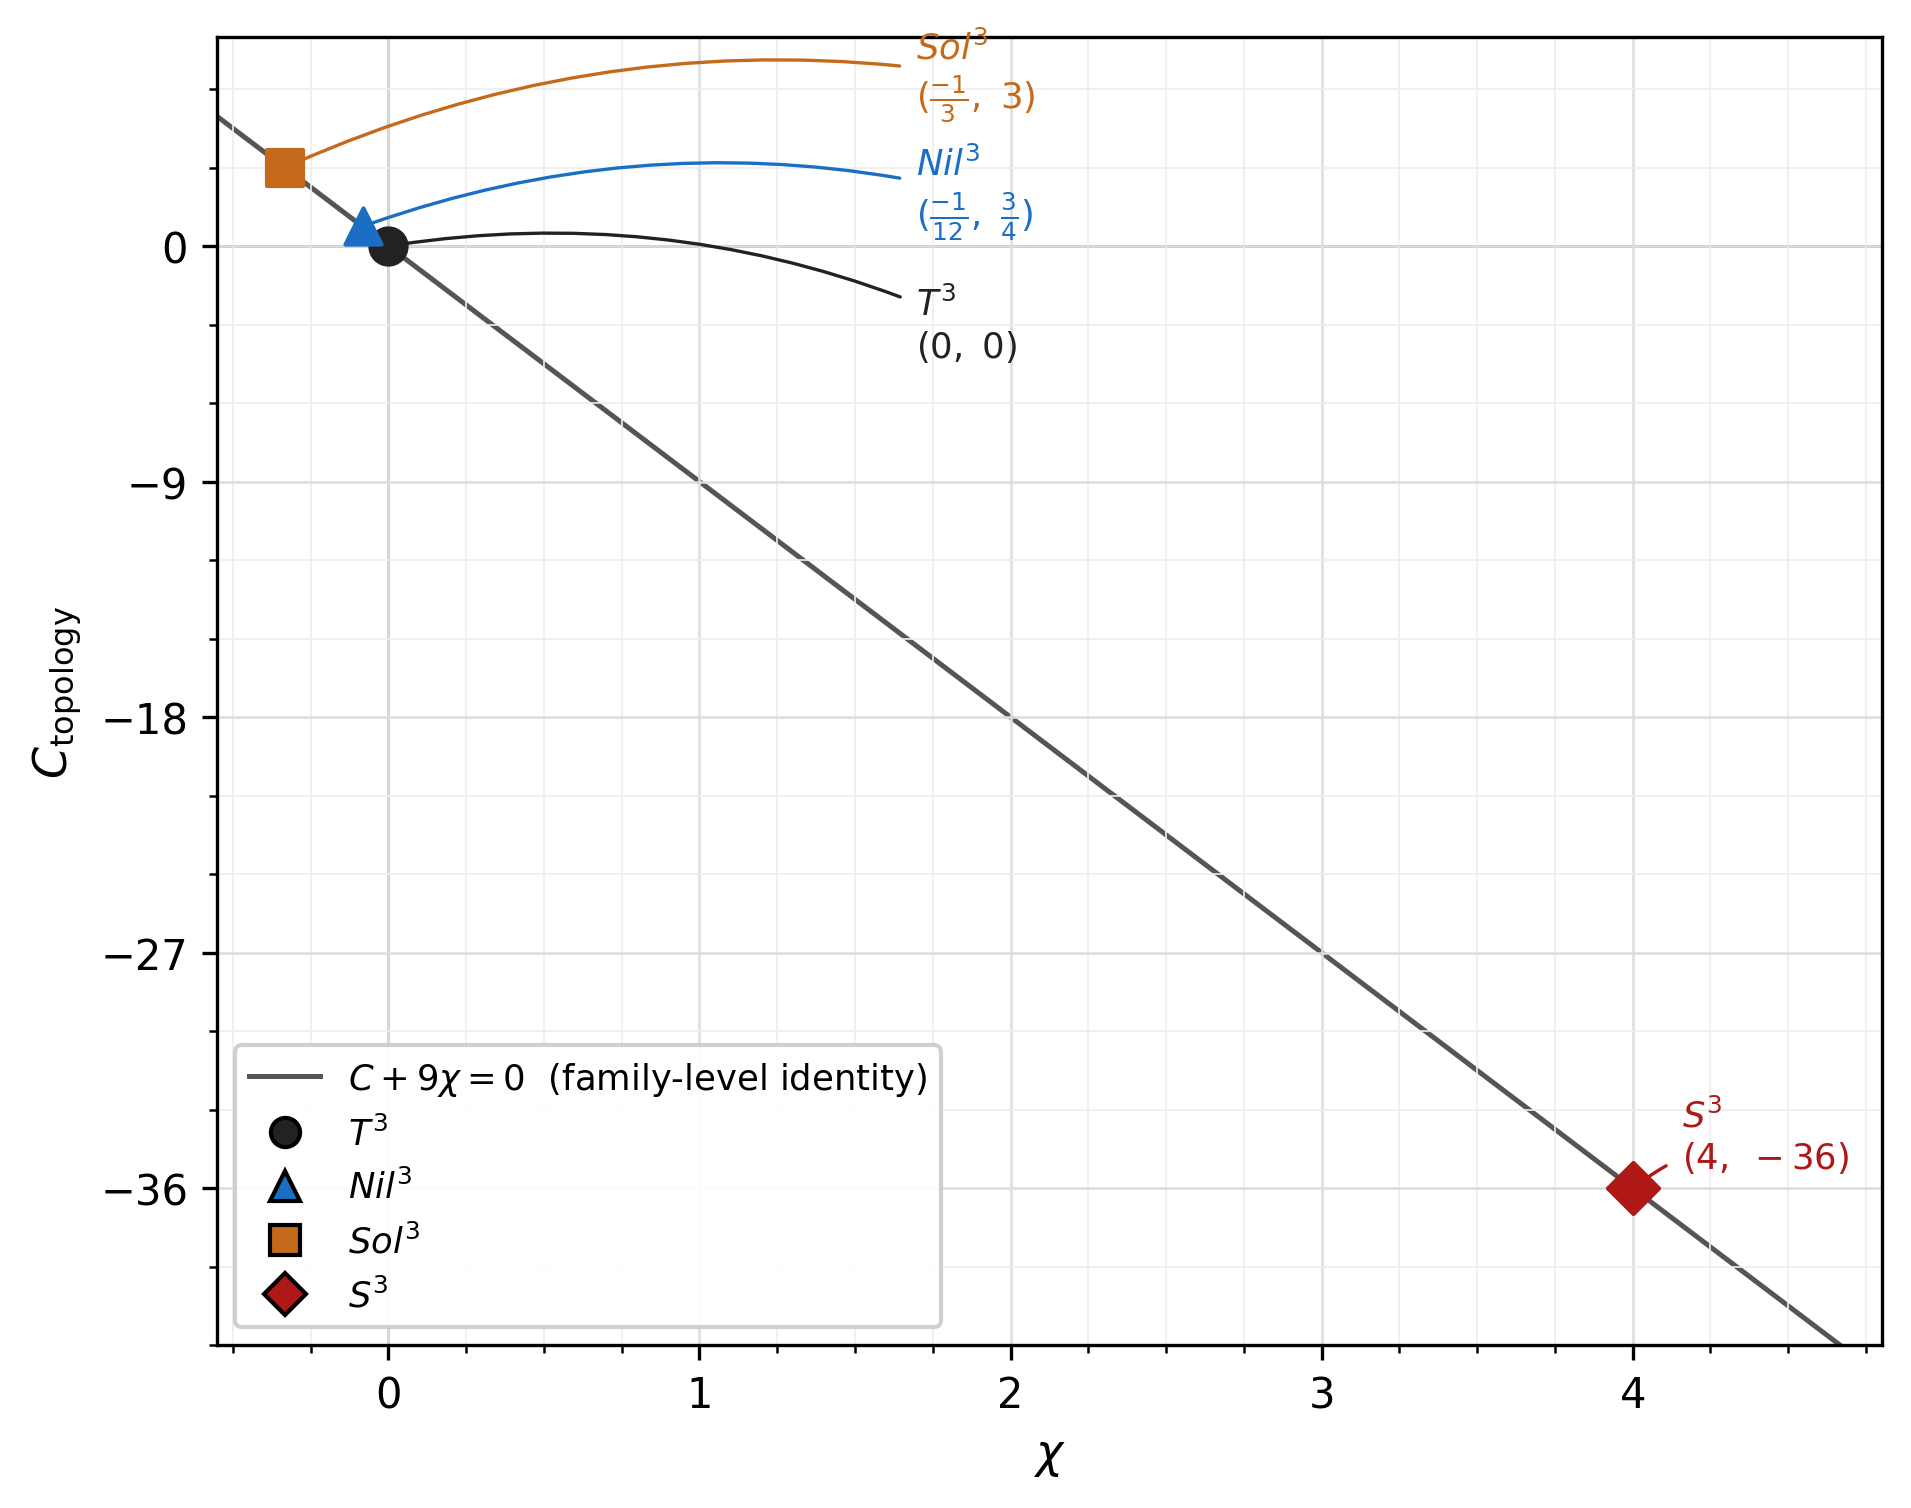
\includegraphics[width=0.9\textwidth]{figures/fig02_chi_bridge_line.png}
  \caption{Diagnostic bridge: the $\Ctop=-9\chi$ line.  The horizontal axis
    is $\chi$ (derived independently from the LC spatial curvature) and the
    vertical axis is $\Ctop$ (extracted from the raw symbolic expression of
    $\PintMX$ by template fitting, without reference to $\chi$).  The four
    points $\Tthree$, $\Nilthree$, $\Solthree$, $\Sthree$ all lie exactly on
    the line $\Ctop+9\chi=0$.  The line is the graphical representation of
    the family-level identity of Section~\ref{sec:bridge:family}; the four
    points are its specialisations.  \emph{Scope}: a family-level identity
    within the LZ-native isotropic $\MX$ sector; $\PintMX$ is an
    internal-pair diagnostic, not a true Pontryagin density.}
  \label{fig:chi_bridge_line}
\end{figure}

The independence of these two quantities deserves emphasis.  As stated in
Section~\ref{sec:pchannel:Pint}, $\Ctop$ is a coefficient extracted from the
raw symbolic expression of $\PintMX$ without reference to $\chi$.  In
contrast, $\chi$ is derived independently from the spatial-curvature sector
as
\begin{equation}
  \chi = \frac{{}^{(3)}R\, q^{2}}{6}.
\end{equation}
Neither computation takes the other quantity as an input, so the relation
$\Ctop = -9\chi$ is not a rephrasing of a definition but the bridge result
between two independent computational routes.

\subsection{Five-parameter family-level identity}
\label{sec:bridge:family}

Over the full five-parameter LZ-native isotropic family of
Section~\ref{sec:setup:chi}, the family-level expression for $\Ctop$ is
\begin{equation}
  \Ctop
  = \frac{3}{4}\,\Disc
  = \frac{3}{4}\!\left(a^{2}-2ab-2ac+b^{2}-2bc+c^{2}
    +4u^{2}+4uv+4v^{2}\right),
\end{equation}
and since $\chi=-\Disc/12$,
\begin{equation}
  \Ctop + 9\chi
  = \frac{3\Disc}{4} - \frac{9\Disc}{12} = 0
\end{equation}
holds as an exact symbolic identity.  This identity is a structural identity
over the entire five-parameter family, not just at the four specific
numerical values of the topologies; the algebraic core is given in
Appendix~\ref{app:B}.

\subsection{Distinguished topology loci}
\label{sec:bridge:loci}

The four topologies are not arbitrary sample points of the five-parameter
family but are located at structurally distinguished loci
(Table~\ref{tab:distinguished_loci}).

\begin{table}[H]
\centering
\resizebox{\linewidth}{!}{%
\begin{tabular}{lcrrll}
\toprule
Topology & $(a,b,c,u,v)$ & $\chi$ & $\Ctop=-9\chi$ & Structural locus & paper~IV echo \\
\midrule
$\Tthree$   & $(0,0,0,0,0)$  & $0$    & $0$  & origin                          & none \\
$\Nilthree$ & $(0,0,-1,0,0)$ & $-1/12$ & $3/4$ & single class-A axis            & uniaxial \\
$\Sthree$   & $(4,4,4,0,0)$  & $4$    & $-36$ & isotropic class-A diagonal     & triaxial \\
$\Solthree$ & $(0,0,0,1,-1)$ & $-1/3$ & $3$  & balanced class-B diagonal pair & biaxial \\
\bottomrule
\end{tabular}%
}
\caption{Distinguished topology loci and paper~IV echo.}
\label{tab:distinguished_loci}
\end{table}

The ``paper~IV echo'' column records an interpretive correspondence with
the KK Higgsing response dictionary of paper~IV (none / uniaxial / triaxial
/ biaxial); details are given in
Section~\ref{sec:discussion:paper04echo}.

\begin{figure}[H]
  \centering
  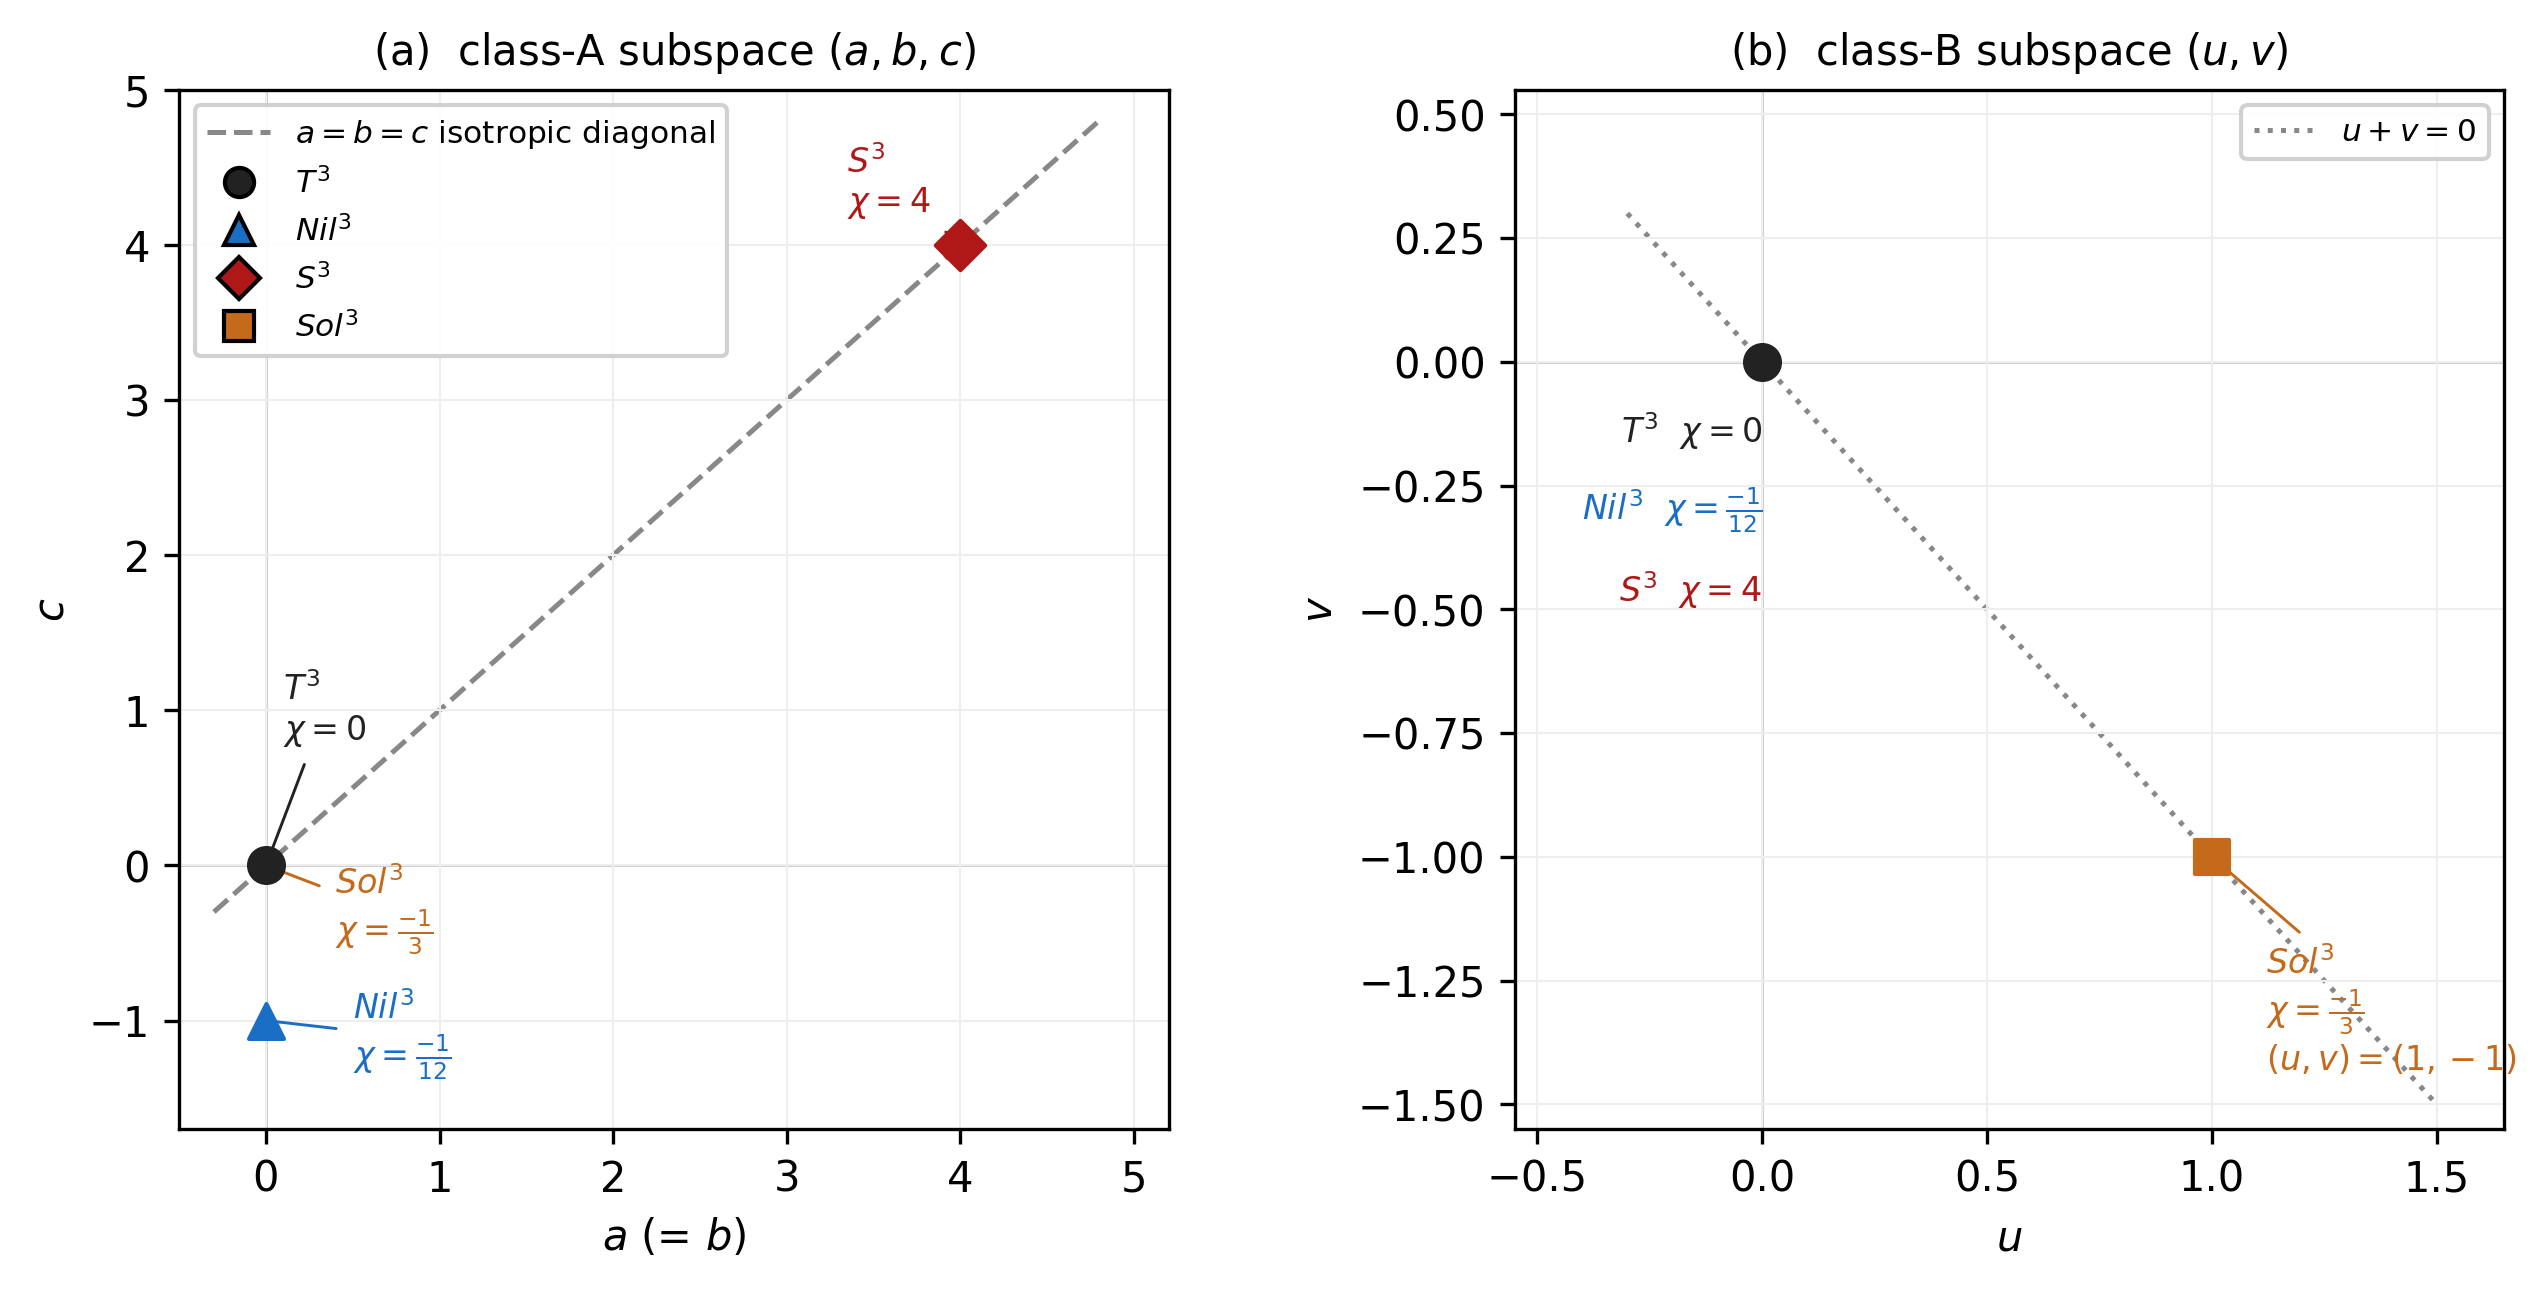
\includegraphics[width=1.0\textwidth]{figures/fig03_loci_diagram.png}
  \caption{Distinguished loci in the five-parameter family
    $(a,b,c,u,v)$.  \textbf{(a) class-A subspace $(a,b,c)$}: all topologies
    lie in the plane $b=a$ and are shown in the $(a,c)$ coordinates.
    $\Tthree$ and $\Solthree$ sit at the class-A origin, $\Nilthree$ on a
    single axis, and $\Sthree$ on the isotropic diagonal $a=b=c$ (dashed).
    \textbf{(b) class-B subspace $(u,v)$}: $\Tthree$, $\Nilthree$, and
    $\Sthree$ collapse to the $u=v=0$ origin, while $\Solthree$ sits at the
    balanced pair $(u,v)=(1,-1)$ on the line $u+v=0$ (dotted).  The four
    points are structurally distinguished loci of the family, not arbitrary
    samples.  \emph{Caveat}: the ``paper~IV echo'' label indicates a
    structural resonance with the paper~IV KK Higgsing dictionary, not an
    identification of the underlying mechanism or theorem
    (see Section~\ref{sec:discussion:paper04echo}).  The present family is
    the LZ-native isotropic $\MX$ family, not a full-theory universal
    family.}
  \label{fig:loci_diagram}
\end{figure}

The scope of $\chi$-universality is restricted to the LZ-native isotropic
$\MX$ reduced sector of this paper.  Extensions to full-theory
universality, arbitrary anisotropic EOM, or matter-coupled sectors are not
claimed here.
   % chi-universality across diagnostic and reduced-orbit levels
%==============================================================================
% Section 6: Four-topology admissibility classification
%==============================================================================
\section{Four-topology admissibility classification}
\label{sec:classification}

The local admissibility classification that integrates the Hamiltonian
admissibility of Section~\ref{sec:hamiltonian} and the P-channel diagnostics
of Section~\ref{sec:pchannel} is collected in
Table~\ref{tab:four_topology_admissibility}.

\begin{table}[H]
\centering
\resizebox{\linewidth}{!}{%
\begin{tabular}{lllll}
\toprule
Topology & $\EH$ & $\AX$ & $\VT$ & $\MX$ \\
\midrule
$\Sthree$   & \code{L_ADMISSIBLE} & \code{L_ADMISSIBLE} & \code{L_ADMISSIBLE} & \code{L_CONDITIONALLY_ADMISSIBLE} \\
$\Tthree$   & \code{L_ADMISSIBLE} & \code{L_ADMISSIBLE} & \code{L_ADMISSIBLE} & \code{L_CONDITIONALLY_ADMISSIBLE} \\
$\Nilthree$ & \code{L_ADMISSIBLE} & \code{L_ADMISSIBLE} & \code{L_ADMISSIBLE} & \code{L_CONDITIONALLY_ADMISSIBLE} \\
$\Solthree$ & \code{L_ADMISSIBLE} & \code{L_ADMISSIBLE} & \code{L_ADMISSIBLE} & \code{L_CONDITIONALLY_ADMISSIBLE} \\
\bottomrule
\end{tabular}%
}
\caption{Four-topology admissibility classification.}
\label{tab:four_topology_admissibility}
\end{table}

The label \code{L_ADMISSIBLE} indicates that the Hamiltonian constraint
closes (Section~\ref{sec:hamiltonian:constraint}), the active-torsion
auxiliary closes (\code{AUX_PASS}), and the diagnostic checks
$\Pform=0$ and $\Pint=0$ are passed.  $\EH$ is a pure-curvature reference
to which the P-channels are not applied.  The label
\code{L_CONDITIONALLY_ADMISSIBLE} indicates that the $\MX$ branch becomes
admissible only under the real-auxiliary-branch condition
$\kap^{4}\thetaNY^{2}+1>0$ and the auxiliary-shell interpretation
$\eta=V=0$.  The off-shell $\PintMX$ and $\QNY$ are recorded as
diagnostic / boundary channels but do not obstruct admissibility.

The structural points of this table can be summarised in three statements.
First, the $\EH$ / $\AX$ / $\VT$ / $\MX$ mode pattern agrees across the
four topologies.  Second, the conditions of the conditional admissibility
of $\MX$ are also common to the four topologies (see the auxiliary
determinant in Section~\ref{sec:hamiltonian:constraint}), so topology does
not change the presence or absence of these conditions.  Third, although
$\Solthree$ carries a caveat regarding the compact quotient
(see Appendix~\ref{app:A}), in the main classification table its row
structure coincides with that of the other three topologies.

This topology-robust pattern is the background for the $\chi$-universality
of Section~\ref{sec:bridge}.  Since admissibility itself does not vary with
topology, topology dependence appears not in the admissibility label but
in the diagnostic / orbit quantities $\Ctop$ and $\chi$.  In this sense,
the bridge result of Section~\ref{sec:bridge} is a natural consequence
that rides on top of the admissibility classification.
   % Four-topology admissibility classification
%==============================================================================
% Section 7: Reduced orbit atlas and chi-sign separation
%==============================================================================
\section{Reduced orbit atlas and $\chi$-sign separation}
\label{sec:orbit}

\subsection{Derivation of the auxiliary-shell orbit equation}
\label{sec:orbit:derivation}

Taking the lapse variation of the reduced action of
Section~\ref{sec:setup:action} gives the Hamiltonian constraint
\begin{equation}
  \dot q^{2} + F_{\topo}(q,\eta,V;\chi) = 0
  \qquad (N=1\ \text{gauge}),
\end{equation}
with the sign in agreement with
Section~\ref{sec:hamiltonian:constraint}.  The auxiliary fields of each
torsion branch are determined algebraically from
$\delta S/\delta\eta=\delta S/\delta V=0$.  The branch functions used in
this paper are
\begin{equation}
  F_{\EH} = \chi,
  \qquad
  F_{\AX} = \chi - \eta^{2},
  \qquad
  F_{\VT} = \chi + \frac{q^{2}V^{2}}{9},
\end{equation}
\begin{equation}
  F_{\MX}
  = \chi - \eta^{2} + \frac{q^{2}V^{2}}{9}
  + \frac{2}{3} qV\eta\,\kap^{2}\thetaNY.
\end{equation}
The auxiliary equations on $\AX$, $\VT$, and $\MX$ give $\eta=0$, $V=0$,
and $(\eta,V)=(0,0)$, respectively.  On $\MX$ we retain the real-branch
condition of Section~\ref{sec:hamiltonian:constraint}.  Therefore, for all
modes and all topologies,
\begin{equation}
  F_{\topo}\big|_{\text{aux-shell}} = \chi
\end{equation}
holds, and we obtain
\begin{equation}
  \boxed{\,\dot q^{2} + \chi = 0\,}.
\end{equation}
This result is obtained independently of the diagnostic-level bridge result
$\Ctop=-9\chi$ of Section~\ref{sec:pchannel:Pint}, and constitutes the
dynamical-side evidence of $\chi$-universality (see
Section~\ref{sec:bridge:two_appearances}).

\subsection{$\chi$-sign separation}
\label{sec:orbit:sign}

Classifying the auxiliary-shell orbit equation by the sign of $\chi$ gives
Table~\ref{tab:chi_sign_atlas}.

\begin{table}[H]
\centering
\begingroup
\renewcommand{\arraystretch}{2.0}
\begin{tabularx}{\linewidth}{llYY}
\toprule
Sign of $\chi$ & \shortstack{Representative\\topology} & \shortstack{Reduced vacuum\\behaviour} & Notes \\
\midrule
$\chi>0$ & $\Sthree$
         & $\dot q^{2}=-\chi<0$: no real initial data
         & A property of the vacuum orbit, independent of the Hamiltonian admissibility (Table~\ref{tab:four_topology_admissibility}) \\
$\chi=0$ & $\Tthree$
         & $\dot q^{2}=0$: static / degenerate
         & Stability discussion is outside the scope of this paper \\
$\chi<0$ & $\Nilthree$, $\Solthree$
         & $\dot q^{2}=-\chi>0$: monotonic expansion and $q\to 0$ singular-approach collapse
         & Orbit classification within the vacuum reduced atlas of this paper \\
\bottomrule
\end{tabularx}
\endgroup
\caption{$\chi$-sign reduced orbit atlas.}
\label{tab:chi_sign_atlas}
\end{table}

\begin{figure}[H]
  \centering
  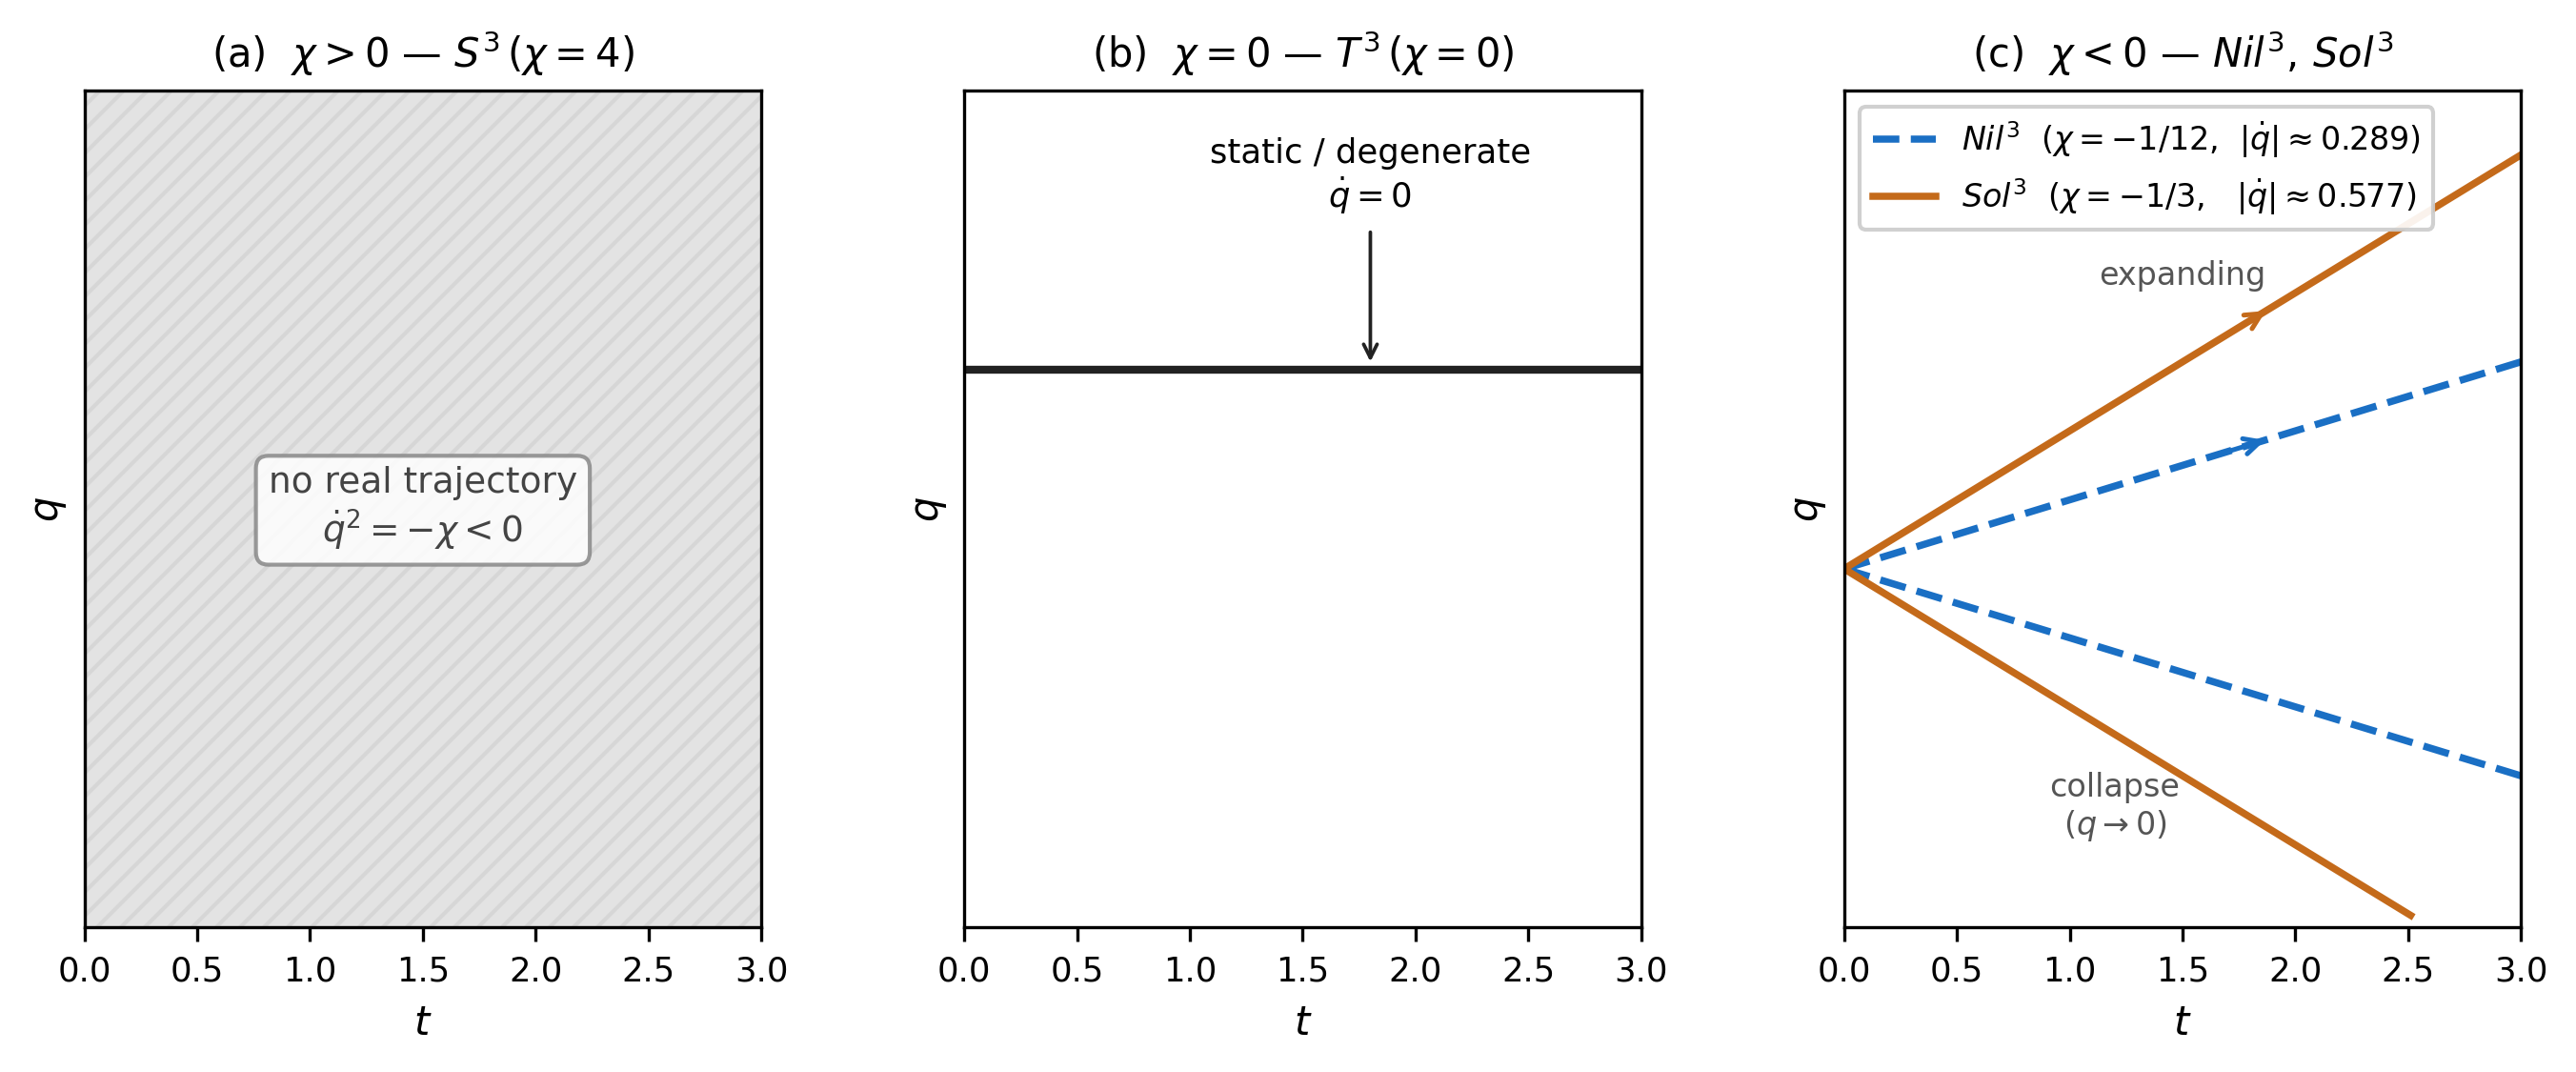
\includegraphics[width=1.0\textwidth]{figures/fig04_chi_sign_orbit_atlas.png}
  \caption{$\chi$-sign reduced orbit atlas, schematic ($q$--$t$ qualitative
    plots).  \textbf{(a) $\chi>0$ ($\Sthree$, $\chi=4$)}: no real initial
    data, since $\dot q^{2}=-\chi<0$ (hatched region).
    \textbf{(b) $\chi=0$ ($\Tthree$, $\chi=0$)}: $\dot q=0$, that is,
    static / degenerate.  \textbf{(c) $\chi<0$ ($\Nilthree$, $\Solthree$)}:
    two sheets $\dot q=\pm\sqrt{-\chi}$ (expanding / collapsing).  The
    slope magnitudes are determined by $|\chi|$:
    $\Nilthree$ gives $|\dot q|=\sqrt{1/12}\approx 0.289$ (dashed) and
    $\Solthree$ gives $|\dot q|=\sqrt{1/3}\approx 0.577$ (solid).
    Bounce-like / recollapse-like classes do not appear in any panel.
    \emph{Caveats}: the figure is a qualitative schematic for the
    constant-velocity solutions of $\dot q^{2}+\chi=0$ and does not include
    an effective potential.  Scope guard: matter coupling, anisotropic, or
    effective-source extensions can change the orbit classes
    (see Section~\ref{sec:orbit:scope} and Appendix~\ref{app:C}).}
  \label{fig:chi_sign_orbit_atlas}
\end{figure}

When $\chi>0$ ($\Sthree$), the absence of real vacuum initial data is a
property of the vacuum reduced atlas, and is independent of the
admissibility classification of
Table~\ref{tab:four_topology_admissibility} (on which $\EH$, $\AX$, $\VT$,
and $\MX$ are all admissible).  The introduction of matter coupling or an
effective source can produce real orbits even on $\Sthree$, but such an
analysis is outside the scope of the present paper.

\subsection{Full-branch sweep summary}
\label{sec:orbit:fullbranch}

The classification of the reduced vacuum orbits across all 16 branches
($\Sthree/\Tthree/\Nilthree/\Solthree$ $\times$ $\EH/\AX/\VT/\MX$) is as
follows.  Each $\chi<0$ branch has two sheets (expanding and collapsing),
so Table~\ref{tab:orbit_class_counts} counts 24 branch/sheet entries
rather than 16 branches.

\begin{table}[H]
\centering
\begin{tabular}{lr}
\toprule
Orbit class & Count \\
\midrule
\code{NO_REAL_AUX_SHELL_ORBIT} & $4$ \\
\code{STATIC_OR_DEGENERATE}    & $4$ \\
\code{MONOTONIC_EXPANSION}     & $8$ \\
\code{SINGULAR_APPROACH}       & $8$ \\
\code{BOUNCE_LIKE}             & $0$ \\
\code{RECOLLAPSE_LIKE}         & $0$ \\
\bottomrule
\end{tabular}
\caption{Full-branch orbit class counts.}
\label{tab:orbit_class_counts}
\end{table}

\code{NO_REAL_AUX_SHELL_ORBIT} reflects the absence of real initial data on
$\Sthree$ ($\chi>0$).  \code{SINGULAR_APPROACH} is the orbit class on the
collapse sheet of $\Nilthree$ and $\Solthree$ ($\chi<0$) for which
$q\to 0$, and is not a statement about finite-time singularities or about
observational cosmology.  Neither class is the same question as the
admissibility classification of
Table~\ref{tab:four_topology_admissibility}.

\subsection{Scope guard}
\label{sec:orbit:scope}

The reduced vacuum atlas considered here contains no \code{BOUNCE_LIKE} or
\code{RECOLLAPSE_LIKE} class.  This is a statement about the vacuum
isotropic reduced setting, and does not extend to matter-coupled,
anisotropic, or effective-source models.  The extensions needed to reach
those settings are discussed in
Section~\ref{sec:discussion:limitations}.
   % Reduced orbit atlas and chi-sign separation
%==============================================================================
% Section 8: Discussion
%==============================================================================
\section{Discussion}
\label{sec:discussion}

\subsection{What $\chi$-universality organises}
\label{sec:discussion:organises}

The results of this paper show that, in the Lorentzian EC+NY reduced
sector, topology dependence is organised by the same scalar $\chi$ across
three levels: Hamiltonian admissibility, P-channel diagnostics, and the
reduced vacuum orbit.

At the admissibility level, the $\EH/\AX/\VT/\MX$ mode pattern is common
to the four topologies (Table~\ref{tab:four_topology_admissibility}), and
the specific values of the topology do not alter the pattern itself.  At
the P-channel level, $\Pform$ is exactly zero independently of topology
(Section~\ref{sec:pchannel:Pform}) and $\QNY$ shows the mode separation
(Section~\ref{sec:pchannel:QNY}); neither has $\chi$-dependence.  Only the
MX diagnostic $\Pint$ distinguishes the topologies, through $\Ctop=-9\chi$
(Section~\ref{sec:pchannel:Pint}).  At the reduced-orbit level, the
auxiliary-shell equation reduces to $\dot q^{2}+\chi=0$
(Section~\ref{sec:orbit:derivation}), and the qualitative classification of
orbits is determined by the sign of $\chi$
(Section~\ref{sec:orbit:sign}).

Taken together, the differences among the four topologies appear in the
reduced sector as differences in the value of the scalar $\chi$, while the
remaining structure (the admissibility pattern, the behaviour of $\Pform$,
and the mode separation) is common across topologies.  We call this
phenomenon $\chi$-controlled topology universality.

\subsection{Relation to the paper~IV response dictionary}
\label{sec:discussion:paper04echo}

The comparison with paper~IV~\cite{paper4} suggests that the four Thurston
geometries used throughout DPPU are not merely a convenient list of
examples.  In paper~IV, these four geometries exhausted four response
types under Euclidean KK Higgsing: none, uniaxial, triaxial, and biaxial.
Here, in a Lorentzian spin-0 / isotropic EC+NY reduction, the same four
geometries appear as structurally distinguished loci of the five-parameter
structure-constant family: the origin ($\Tthree$), a single class-A axis
($\Nilthree$), the isotropic class-A diagonal ($\Sthree$), and a balanced
class-B pair ($\Solthree$).  The $\chi$-universality result therefore
provides a new reading of the same four-geometry response dictionary in a
different reduced sector, rather than a direct identification with the
paper~IV mechanism.

These two results suggest that the same set of Thurston geometries gives a
coherent classificatory structure across different reduced sectors of DPPU
theory, but the elucidation of a common underlying basis is left to
future work.

\subsection{Limitations and future directions}
\label{sec:discussion:limitations}

This paper is restricted to the $\alpha=0$ EC+NY isotropic reduced sector,
and the following extensions are explicitly left to future work.

For $\Nilthree$ and $\Solthree$, this paper uses only the reduced
description in terms of the isotropic scale $q$ and does not derive the
anisotropic EOM with independent scale factors.  For $\Solthree$, the
construction of compact quotients, the classification of spin structures,
and the determination of spectral data are outside the scope of the
present paper.  The absence of real initial data on the $\Sthree$ vacuum
reduced atlas may be resolved by the introduction of matter coupling or an
effective source, but that analysis is outside the scope of the present
paper.  As for the Weyl-source / $\alpha\neq0$ branches, this paper is
restricted to the $\alpha=0$ baseline and does not include a re-evaluation
of the other branches.

For the exact cancellation of $\Pform$ by block orthogonality and the
$\chi$-specialisation of $\PintMX$, we present the results as confirmed by
symbolic computation, and do not proceed to abstract formulation in the
form of formal lemmas and propositions.

\subsection{Closing remarks}
\label{sec:discussion:closing}

In summary, this paper has shown that in the Lorentzian EC+NY reduced
sector the four topologies $\Sthree$, $\Tthree$, $\Nilthree$, $\Solthree$
share a common admissibility pattern, and that the topology dependence is
collapsed onto a single scalar $\chi$ through two independent routes: the
diagnostic identity $\Ctop=-9\chi$ and the reduced vacuum orbit
$\dot q^{2}+\chi=0$.  This $\chi$-controlled topology universality is a
classification result in the reduced sector; generalisation to
anisotropic, matter-coupled, and global extensions is a future task
beyond the scope of the present paper.
   % Discussion

%------------------------------------------------------------------------------
% Acknowledgments
%------------------------------------------------------------------------------
\section*{Acknowledgments}

The author acknowledges the use of the following AI tools during manuscript
preparation: Claude Opus~4.7 (Anthropic; accessed 2026-05),
Gemini~3.1 Pro (Google; accessed 2026-05), Grok~4.3 (xAI; accessed 2026-05),
and GPT-5.5 Thinking via ChatGPT (OpenAI; accessed 2026-05).
These tools were used for language editing (including Japanese--English
translation), outlining and improving exposition, drafting and reviewing
auxiliary code (scripts and pseudocode) that was subsequently tested and
validated by the author, and proposing candidate consistency checks and
alternative derivations to be independently verified by the author.

The AI tools did not determine the scientific claims of this work and were not
used to generate or modify research data or evidentiary figures.  The author
takes full responsibility for the content and for any remaining errors.

This work was developed within the informal collaborative project
\textbf{DPPU} (\textbf{D}onut-like topology, \textbf{P}lanck-scale
compactness, \textbf{P}recession dynamics, \textbf{U}niverse).

%------------------------------------------------------------------------------
% Availability and Contact
%------------------------------------------------------------------------------
\section*{Availability and Contact}

\paragraph{Code and Data Availability}
The code and supplemental data associated with this work are available at:

\begin{itemize}
  \item Zenodo: 10.5281/zenodo.20228881
  \item GitHub: \texttt{https://github.com/Muacca/DPPUv7-paper06}
\end{itemize}

They are released under the MIT License.

\paragraph{Citation}
If you use these materials, please cite the associated manuscript and Zenodo
record:

\begin{quote}
\small
Muacca, ``Reduced-Sector $\chi$-Universality in Lorentzian EC+NY
Minisuperspace: Topology-Robust Admissibility, P-Channel Diagnostics,
and Reduced Vacuum Orbits.''
\end{quote}

\paragraph{Contact}
For questions, bug reports, or collaboration inquiries:

\begin{itemize}
  \item Email: \texttt{muacca@dmwp.jp}
  \item GitHub Issues: \texttt{https://github.com/Muacca/DPPUv7-paper06/issues}
\end{itemize}

%------------------------------------------------------------------------------
% Appendices
%------------------------------------------------------------------------------
\appendix
%==============================================================================
% Appendix A: Topology conventions, local reductions, and caveats
%==============================================================================
\section{Topology conventions, local reductions, and caveats}
\label{app:A}

\subsection{Structure constants and $\chi$ values}
\label{app:A:structure}

The spatial structure constants for the four topologies are given as
specialisations of the five-parameter LZ-native isotropic family.  The
family parameters are $(a,b,c,u,v)$, and the antisymmetrised structure
constants are defined by
\begin{equation}
  C^{1}{}_{23}=\frac{a}{q},\quad
  C^{2}{}_{31}=\frac{b}{q},\quad
  C^{3}{}_{12}=\frac{c}{q},\quad
  C^{2}{}_{12}=\frac{u}{q},\quad
  C^{3}{}_{13}=\frac{v}{q}.
\end{equation}
The three-dimensional Ricci scalar then reads
\begin{equation}
  {}^{(3)}R\,q^{2} = -\tfrac{1}{2}\,\Disc,
  \qquad
  \Disc = a^{2}-2ab-2ac+b^{2}-2bc+c^{2}+4u^{2}+4uv+4v^{2},
\end{equation}
and the $\chi$ of this paper is defined by
\begin{equation}
  \chi = -\frac{\Disc}{12}.
\end{equation}
The parameter values and $\chi$ values for each topology are listed in
Table~\ref{tab:appA_topology}.

\begin{table}[H]
\centering
\begingroup
\renewcommand{\arraystretch}{2.0}
\begin{tabularx}{\linewidth}{lcrrYY}
\toprule
Topology & $(a,b,c,u,v)$ & $\Disc$ & $\chi$ & Reduction status & Caveat \\
\midrule
$\Sthree$   & $(4,4,4,0,0)$  & $-48$ & $4$     & closed isotropic reference   & --- \\
$\Tthree$   & $(0,0,0,0,0)$  & $0$   & $0$     & flat reference               & --- \\
$\Nilthree$ & $(0,0,-1,0,0)$ & $1$   & $-1/12$ & isotropic-scale local branch & anisotropic EOM left to future work \\
$\Solthree$ & $(0,0,0,1,-1)$ & $4$   & $-1/3$  & isotropic-scale local branch & compact quotient outside the scope of this paper \\
\bottomrule
\end{tabularx}
\endgroup
\caption{Topology conventions, $\chi$ values, and reduction status.}
\label{tab:appA_topology}
\end{table}

\paragraph{Verification.}
$\Sthree$: $\Disc=(16-32-32+16-32+16)=-48$, $\chi=4$.
$\Nilthree$: $\Disc=1$, $\chi=-1/12$.
$\Solthree$: $\Disc=(4-4+4)=4$, $\chi=-1/3$.

\subsection{Distinguished loci in the five-parameter family}
\label{app:A:loci}

Table~\ref{tab:appA_loci} records, on top of the topology ordering and the
$(\Disc,\chi)$ conventions fixed in Table~\ref{tab:appA_topology}, only the
additional bridge-facing information.  Here $\Ctop$ is computed from
$\Ctop = 3\Disc/4$ of Appendix~\ref{app:B:bridge}, and each row satisfies
$\Ctop+9\chi=0$.

\begin{table}[H]
\centering
\begin{tabular}{lrll}
\toprule
Topology & $\Ctop=3\Disc/4$ & Structural locus & paper~IV echo \\
\midrule
$\Sthree$   & $-36$ & isotropic class-A diagonal      & triaxial \\
$\Tthree$   & $0$   & origin                          & none \\
$\Nilthree$ & $3/4$ & single class-A axis             & uniaxial \\
$\Solthree$ & $3$   & balanced class-B diagonal pair  & biaxial \\
\bottomrule
\end{tabular}
\caption{Bridge-facing structural loci.}
\label{tab:appA_loci}
\end{table}

The paper~IV echo column is interpretive only.  It records a structural
resonance with the response dictionary of paper~IV, not an equivalence of
mechanisms or a shared theorem.

\subsection{Reduction scope for $\Nilthree$ and $\Solthree$}
\label{app:A:reduction}

$\Nilthree$ is the non-Abelian homogeneous geometry determined by the
left-invariant metric on the Heisenberg
group~\cite{Thurston1997,Scott1983}; the sign convention adopted here is
$C^{3}{}_{12}=-1/q$ (that is, $c=-1$).  Under the isotropic-scale reduction
a single scale parameter $q$ is shared across all directions.  The
anisotropic EOM obtained by introducing independent scale factors is not
derived in this paper.

$\Solthree$ is the geometry based on a solvable Lie
group~\cite{Thurston1997,Scott1983} and enters the five-parameter family
as a balanced class-B diagonal pair $u=1$, $v=-1$.  This is the
isotropic-scale reduced entry of the present paper.  A compact realisation
of $\Solthree$ requires a mapping-torus construction; the choice of lattice
normalisation, the classification of spin structures, and the determination
of spectral data are outside the scope of the present paper.  The
$\Solthree$ entries of Table~\ref{tab:four_topology_admissibility} and
Table~\ref{tab:chi_sign_atlas} are restricted to this local / isotropic
reduced branch.

\subsection{Lorentzian EC+NY action conventions}
\label{app:A:action}

We adopt the orthonormal frame in Lorentzian signature $(-,+,+,+)$, and the
Nieh--Yan coupling is parametrised by real $\thetaNY$.  The frame
block-diagonal structure of $\Pform$ is common to the Lorentzian and
Euclidean settings, but the sign convention of the Hamiltonian constraint
follows the Lorentzian convention
(Section~\ref{sec:hamiltonian:constraint}).  The definition of $\Pint$ and
the orientation of $\QNY$ inherit the conventions of
paper~V~\cite{paper5}.

The constant term $\Ctop=-36$ of the $\Sthree$ specialisation agrees with
the constant term of the $\MX$-$P$ expression of paper~III (``Unified
Geometric Landau EFT'')~\cite{paper3}.  On the other hand, the sign of the
$V^{2}q^{2}$ term originates from the difference between the Euclidean
convention of paper~III~\cite{paper3} and the Lorentzian metric-aware
epsilon / legacy temporal-index map of the present paper.
  % Topology conventions, local reductions, and caveats
%==============================================================================
% Appendix B: Computational checks and reproducibility
%==============================================================================
\section{Computational checks and reproducibility}
\label{app:B}

\subsection{Algebraic core of the $\chi$-bridge identity}
\label{app:B:bridge}

We record the algebraic core of the family-level identity
$\Ctop+9\chi=0$ of Section~\ref{sec:bridge:family}.  With the auxiliary
quantity $\Disc$ defined as
\begin{equation}
  \Disc = a^{2}-2ab-2ac+b^{2}-2bc+c^{2}+4u^{2}+4uv+4v^{2},
\end{equation}
the two quantities $\chi$ and $\Ctop$ are expressed as
\begin{equation}
  \chi = -\frac{\Disc}{12},
  \qquad
  \Ctop = \frac{3\Disc}{4}.
\end{equation}
Then
\begin{equation}
  \Ctop + 9\chi = \frac{3\Disc}{4} - \frac{9\Disc}{12} = 0.
\end{equation}
This identity holds for arbitrary values of $\Disc$ and does not assume any
specific topology.  The specialised values for the four topologies
(Table~\ref{tab:appA_topology}) are substitutions into this identity.

\subsection{Full topology branch taxonomy}
\label{app:B:branch_taxonomy}

The main admissibility classification across all 16 branches
($\Sthree/\Tthree/\Nilthree/\Solthree$ $\times$ $\EH/\AX/\VT/\MX$) is
given in Table~\ref{tab:appB1}.  Table~\ref{tab:four_topology_admissibility}
(Section~\ref{sec:classification}) is the summary of this classification
pattern.  The full $F$-branch expressions, the Hamiltonian constraints,
the auxiliary equations, and the auxiliary-shell solutions can be
reproduced with \code{admissibility_classification.py}.

\begin{table}[H]
\centering
\resizebox{\linewidth}{!}{%
\begin{tabular}{llcccl}
\toprule
Topology & Mode & $\chi$ & $F_{\mathrm{shell}}$ & Hessian determinant & Label \\
\midrule
$\Sthree$   & $\EH$ & $4$ & $4$ & n/a & \code{L_ADMISSIBLE} \\
$\Sthree$   & $\AX$ & $4$ & $4$ & $-2$ & \code{L_ADMISSIBLE} \\
$\Sthree$   & $\VT$ & $4$ & $4$ & $2q^{2}/9$ & \code{L_ADMISSIBLE} \\
$\Sthree$   & $\MX$ & $4$ & $4$ & $-4q^{2}(\kap^{4}\thetaNY^{2}+1)/9$ & \code{L_CONDITIONALLY_ADMISSIBLE} \\
$\Tthree$   & $\EH$ & $0$ & $0$ & n/a & \code{L_ADMISSIBLE} \\
$\Tthree$   & $\AX$ & $0$ & $0$ & $-2$ & \code{L_ADMISSIBLE} \\
$\Tthree$   & $\VT$ & $0$ & $0$ & $2q^{2}/9$ & \code{L_ADMISSIBLE} \\
$\Tthree$   & $\MX$ & $0$ & $0$ & $-4q^{2}(\kap^{4}\thetaNY^{2}+1)/9$ & \code{L_CONDITIONALLY_ADMISSIBLE} \\
$\Nilthree$ & $\EH$ & $-1/12$ & $-1/12$ & n/a & \code{L_ADMISSIBLE} \\
$\Nilthree$ & $\AX$ & $-1/12$ & $-1/12$ & $-2$ & \code{L_ADMISSIBLE} \\
$\Nilthree$ & $\VT$ & $-1/12$ & $-1/12$ & $2q^{2}/9$ & \code{L_ADMISSIBLE} \\
$\Nilthree$ & $\MX$ & $-1/12$ & $-1/12$ & $-4q^{2}(\kap^{4}\thetaNY^{2}+1)/9$ & \code{L_CONDITIONALLY_ADMISSIBLE} \\
$\Solthree$ & $\EH$ & $-1/3$ & $-1/3$ & n/a & \code{L_ADMISSIBLE} \\
$\Solthree$ & $\AX$ & $-1/3$ & $-1/3$ & $-2$ & \code{L_ADMISSIBLE} \\
$\Solthree$ & $\VT$ & $-1/3$ & $-1/3$ & $2q^{2}/9$ & \code{L_ADMISSIBLE} \\
$\Solthree$ & $\MX$ & $-1/3$ & $-1/3$ & $-4q^{2}(\kap^{4}\thetaNY^{2}+1)/9$ & \code{L_CONDITIONALLY_ADMISSIBLE} \\
\bottomrule
\end{tabular}%
}
\caption{Compact full branch taxonomy.}
\label{tab:appB1}
\end{table}

\subsection{Full orbit-sheet atlas}
\label{app:B:orbit_atlas}

The 24 branch/sheet rows of the reduced vacuum orbit atlas are given in
Table~\ref{tab:appB2}.  $\Sthree$ and $\Tthree$ contribute one row per
branch, while $\Nilthree$ and $\Solthree$ contribute two sheets
(expanding / collapsing).  Table~\ref{tab:orbit_class_counts}
(Section~\ref{sec:orbit:fullbranch}) summarises this branch/sheet count.
The orbit equations, constraint residuals, and numerical monitors of each
row can be reproduced with \code{orbit_atlas.py}.

\begin{table}[H]
\centering
\resizebox{\linewidth}{!}{%
\begin{tabular}{lllllc}
\toprule
Topology & Mode & Sheet & $\dot q_{0}$ & Orbit class & Check \\
\midrule
$\Sthree$   & $\EH$ & none       & no real solution & \code{NO_REAL_AUX_SHELL_ORBIT} & PASS \\
$\Sthree$   & $\AX$ & none       & no real solution & \code{NO_REAL_AUX_SHELL_ORBIT} & PASS \\
$\Sthree$   & $\VT$ & none       & no real solution & \code{NO_REAL_AUX_SHELL_ORBIT} & PASS \\
$\Sthree$   & $\MX$ & none       & no real solution & \code{NO_REAL_AUX_SHELL_ORBIT} & PASS \\
$\Tthree$   & $\EH$ & zero       & $0$              & \code{STATIC_OR_DEGENERATE}    & PASS \\
$\Tthree$   & $\AX$ & zero       & $0$              & \code{STATIC_OR_DEGENERATE}    & PASS \\
$\Tthree$   & $\VT$ & zero       & $0$              & \code{STATIC_OR_DEGENERATE}    & PASS \\
$\Tthree$   & $\MX$ & zero       & $0$              & \code{STATIC_OR_DEGENERATE}    & PASS \\
$\Nilthree$ & $\EH$ & expanding  & $\sqrt{3}/6$     & \code{MONOTONIC_EXPANSION}     & PASS \\
$\Nilthree$ & $\EH$ & collapsing & $-\sqrt{3}/6$    & \code{SINGULAR_APPROACH}       & PASS \\
$\Nilthree$ & $\AX$ & expanding  & $\sqrt{3}/6$     & \code{MONOTONIC_EXPANSION}     & PASS \\
$\Nilthree$ & $\AX$ & collapsing & $-\sqrt{3}/6$    & \code{SINGULAR_APPROACH}       & PASS \\
$\Nilthree$ & $\VT$ & expanding  & $\sqrt{3}/6$     & \code{MONOTONIC_EXPANSION}     & PASS \\
$\Nilthree$ & $\VT$ & collapsing & $-\sqrt{3}/6$    & \code{SINGULAR_APPROACH}       & PASS \\
$\Nilthree$ & $\MX$ & expanding  & $\sqrt{3}/6$     & \code{MONOTONIC_EXPANSION}     & PASS \\
$\Nilthree$ & $\MX$ & collapsing & $-\sqrt{3}/6$    & \code{SINGULAR_APPROACH}       & PASS \\
$\Solthree$ & $\EH$ & expanding  & $\sqrt{3}/3$     & \code{MONOTONIC_EXPANSION}     & PASS \\
$\Solthree$ & $\EH$ & collapsing & $-\sqrt{3}/3$    & \code{SINGULAR_APPROACH}       & PASS \\
$\Solthree$ & $\AX$ & expanding  & $\sqrt{3}/3$     & \code{MONOTONIC_EXPANSION}     & PASS \\
$\Solthree$ & $\AX$ & collapsing & $-\sqrt{3}/3$    & \code{SINGULAR_APPROACH}       & PASS \\
$\Solthree$ & $\VT$ & expanding  & $\sqrt{3}/3$     & \code{MONOTONIC_EXPANSION}     & PASS \\
$\Solthree$ & $\VT$ & collapsing & $-\sqrt{3}/3$    & \code{SINGULAR_APPROACH}       & PASS \\
$\Solthree$ & $\MX$ & expanding  & $\sqrt{3}/3$     & \code{MONOTONIC_EXPANSION}     & PASS \\
$\Solthree$ & $\MX$ & collapsing & $-\sqrt{3}/3$    & \code{SINGULAR_APPROACH}       & PASS \\
\bottomrule
\end{tabular}%
}
\caption{Compact full orbit-sheet atlas.}
\label{tab:appB2}
\end{table}

\subsection{Summary of main computational checks}
\label{app:B:checks}

Table~\ref{tab:appB3} lists the logical verification targets.  The first
two checks are evaluated by the same symbolic script, because the
family-level identity and its topology specialisations share the same
derived $(a,b,c,u,v)$ data.

\begin{table}[H]
\centering
\begingroup
\renewcommand{\arraystretch}{2.0}
\begin{tabularx}{\linewidth}{YYYY}
\toprule
Check & Content & \shortstack{Related\\section} & Script \\
\midrule
$\chi$-bridge derivation
  & Extract $(a,b,c,u,v)$ for $\Sthree/\Tthree/\Nilthree/\Solthree$,
    derive $\chi$ from the LC spatial curvature, compute the raw $\PintMX$
    from the EC+NY MX curvature, and extract $\Ctop$
  & Section~\ref{sec:pchannel:Pint}, \ref{sec:bridge:family}
  & \code{chi_bridge_symbolic.py} \\
$\Pform$ cancellation
  & Construct the curvature with the EC+NY engine for each torsion branch
    $\AX/\VT/\MX$ and compute $\Pform$
  & Section~\ref{sec:pchannel:Pform}
  & \code{pform_cancellation.py} \\
admissibility classification
  & Derive the lapse constraint and the auxiliary closure symbolically from
    the engine-derived $F_{\mathrm{branch}}$
  & Section~\ref{sec:hamiltonian}, \ref{sec:classification}
  & \code{admissibility_classification.py} \\
orbit atlas
  & Derive the orbit equation and the orbit class from the auxiliary
    shell of the engine-derived $F_{\mathrm{branch}}$
  & Section~\ref{sec:orbit}
  & \code{orbit_atlas.py} \\
\bottomrule
\end{tabularx}
\endgroup
\caption{Computational checks and their roles.}
\label{tab:appB3}
\end{table}
  % Tables, computational checks, and reproducibility notes
%==============================================================================
% Appendix C: Bianchi I lite comparison and reduced-atlas scope
%==============================================================================
\section{Bianchi I lite comparison and reduced-atlas scope}
\label{app:C}

\subsection{Purpose}
\label{app:C:purpose}

The purpose of this appendix is to make explicit the scope of the present
paper by clarifying the structural differences between the reduced vacuum
atlas of this paper and Bianchi~I / Nieh--Yan-type systems.

\subsection{Structural comparison}
\label{app:C:comparison}

The reduced orbit equation of this paper is $\dot q^{2}+\chi=0$, which
contains only the isotropic scale $q$ and the topology scalar $\chi$.  It
contains neither matter coupling nor effective-source terms.  In contrast,
the Bianchi~I / NY-type bounce-like
systems~\cite{BrandenbergerPeter2017} typically involve several
independent scale factors, matter sources, and effective potentials, and
the existence of a turning point ($\dot q=0$, $\ddot q>0$) is a necessary
condition for the realisation of a bounce-like orbit.

\begin{table}[H]
\centering
\resizebox{\linewidth}{!}{%
\begin{tabular}{lll}
\toprule
Item & Present reduced orbit atlas & Bianchi~I / NY type \\
\midrule
Orbit equation & $\dot q^{2}+\chi=0$ & involves a richer effective potential \\
Scale factor & isotropic scalar $q$ & generally several independent factors \\
Matter coupling & none & generally present \\
Bounce-like turning point & not found in the present scope & depends on the potential \\
Geometric basis & Thurston geometry $\times$ EC+NY torsion & model-dependent \\
\bottomrule
\end{tabular}%
}
\caption{Structural comparison with Bianchi~I lite.}
\label{tab:appC_bianchi}
\end{table}

This comparison is a sanity benchmark, not a matching of the same model.

\subsection{Scope statement}
\label{app:C:scope}

The absence of \code{BOUNCE_LIKE} and \code{RECOLLAPSE_LIKE} orbit classes
in the vacuum reduced atlas of the present paper is a property of this
isotropic vacuum reduced setting.  This result is not a general no-go
claim against matter-coupled, effective-source, or anisotropic extensions.
For instance, on $\Sthree$ ($\chi>0$) the absence of real initial data on
the vacuum reduced atlas is not a denial that the introduction of a matter
source -- changing the structure of the Hamiltonian constraint -- could
permit bounce-like orbits~\cite{BrandenbergerPeter2017}.  The analysis of
these extensions is a future task.
  % Bianchi I lite comparison and reduced-atlas scope guard

%------------------------------------------------------------------------------
% References
%------------------------------------------------------------------------------
\bibliographystyle{unsrt}

\begin{thebibliography}{99}

\bibitem{paper1}
Muacca,
``Topology-Dependent Phase Classification of Effective Potentials
in Einstein--Cartan + Nieh--Yan Minisuperspace,''
Zenodo.\ \texttt{10.5281/zenodo.18213677} (2026).

\bibitem{paper2}
Muacca,
``Structural Robustness of Isotropic $\Sthree$ Vacua in
Einstein--Cartan Minisuperspace via Chiral Equilibrium and Weyl Stability,''
Zenodo.\ \texttt{10.5281/zenodo.18815498} (2026).

\bibitem{paper3}
Muacca,
``Unified Geometric Landau EFT of Homogeneous $\Sthree\times S^{1}$
Minisuperspace in Einstein--Cartan + Nieh--Yan Theory,''
Zenodo.\ \texttt{10.5281/zenodo.19144481} (2026).

\bibitem{paper3ec}
Muacca,
``Homogeneous Three-Topology Comparison and Mode Dictionary
in Einstein--Cartan + Nieh--Yan Theory: Geometric Structure of EC--Weyl
Coupling,''
Zenodo.\ \texttt{10.5281/zenodo.19425147} (2026).

\bibitem{paper4}
Muacca,
``Euclidean Geometric Response Dictionary and Selection Rules
for Four Thurston Geometries,''
Zenodo.\ \texttt{10.5281/zenodo.19775695} (2026).

\bibitem{paper5}
Muacca,
``Lorentzian Einstein--Cartan Minisuperspace with Nieh--Yan Torsion:
Hamiltonian Branches, Pontryagin Diagnostics,
and Weyl-Source Obstructions,''
Zenodo.\ \texttt{10.5281/zenodo.20084722} (2026).

\bibitem{Hehl1976}
F.~W.~Hehl, P.~von der Heyde, G.~D.~Kerlick, and J.~M.~Nester,
``General relativity with spin and torsion: Foundations and prospects,''
Rev.\ Mod.\ Phys.\ \textbf{48}, 393--416 (1976).

\bibitem{NiehYan1982}
H.~T.~Nieh and M.~L.~Yan,
``An identity in Riemann--Cartan geometry,''
J.\ Math.\ Phys.\ \textbf{23}, 373--374 (1982).

\bibitem{Thurston1997}
W.~P.~Thurston,
\emph{Three-Dimensional Geometry and Topology, Volume 1},
edited by S.~Levy
(Princeton University Press, Princeton, NJ, 1997).

\bibitem{Scott1983}
P.~Scott,
``The geometries of 3-manifolds,''
Bull.\ London Math.\ Soc.\ \textbf{15}, 401--487 (1983).

\bibitem{EllisMacCallum1969}
G.~F.~R.~Ellis and M.~A.~H.~MacCallum,
``A class of homogeneous cosmological models,''
Commun.\ Math.\ Phys.\ \textbf{12}, 108--141 (1969).

\bibitem{BrandenbergerPeter2017}
R.~Brandenberger and P.~Peter,
``Bouncing Cosmologies: Progress and Problems,''
Found.\ Phys.\ \textbf{47}, 797--850 (2017),
arXiv:1603.05834, doi:10.1007/s10701-016-0057-0.

\bibitem{ChandiaZanelli1997}
O.~Chandia and J.~Zanelli,
``Topological invariants, instantons, and the chiral anomaly on spaces with
torsion,''
Phys.\ Rev.\ D \textbf{55}, 7580--7585 (1997).

\end{thebibliography}

%==============================================================================
\end{document}
%==============================================================================
